\section{Preliminaries}\label{sec:prelims}
In this section, we establish a few basic definitions and results that will be used throughout the rest of the paper. As mentioned above, several results in this section are already proved in \cite{postle2016five} for list colouring instead of correspondence colouring. In all cases, the results are easily adapted for correspondence colouring. In the interest of brevity, we have omitted the proofs that are identical to those given in \cite{postle2016five}. As mentioned in Section \ref{sec:challenges}, whenever this is the case, the proofs in question are purely structural and do not mention colourings at all.

\subsection{Critical Subgraphs}\label{subsec:criticalgraph}
In this subsection, we establish a few basic properties of \emph{critical canvases}, the main object under study. We will need the following definitions.

\begin{definition}
Let $G$ be a graph. For a set $X \subseteq V(G)$, we denote by $N(X)$ the set $\left(\bigcup_{v \in X} N(v) \right) \setminus X$. 
\end{definition}


\begin{definition}[$S$-critical]
Let $G$ be a graph, $S \subseteq G$ a subgraph of $G$, and $(L,M)$ a correspondence assignment for $G$. For an $(L,M)$-colouring $\phi$ of $S$, we say that \emph{$\phi$ extends to an $(L,M)$-colouring} of $G$ if there exists an $(L,M)$-colouring $\psi$ of $G$ such that $\phi(v)=\psi(v)$ for all $v\in V(S)$.  The graph $G$ is \emph{$S$-critical with respect to $(L,M)$} if $G \ne S$ and for every proper subgraph $G' \subset G$ such that $S \subseteq G'$, there exists an $(L,M)$-colouring of $S$ that extends to an $(L,M)$-colouring of $G'$, but does not extend to an $(L,M)$-colouring of $G$. If the list assignment is clear from the context, we shorten this and say that $G$ is $S$-critical.
\end{definition}

\begin{definition}
\label{def:canvas}
We say the triple $(G,C,(L,M))$ is a \emph{canvas} if $G$ is a $2$-connected plane graph, $C$ is its outer cycle, and $(L,M)$ is a correspondence assignment for the vertices of $G$ such that $|L(v)|\ge 5$ for all $v\in V(G)\setminus V(C)$ and there exists an $(L,M)$-colouring of $C$. We say a canvas $(G,C,(L,M))$ is \emph{critical} if $G$ is $C$-critical with respect to the correspondence assignment $(L,M)$.
\end{definition}
These definitions match those given for list colouring in \cite{postle2016five}, with the appropriate adjustments for correspondence colouring instead of list colouring.

In addition to being used below to establish helpful corollaries regarding subgraphs of critical canvases, the following lemma will be used in Section \ref{sec:implications} to show that the family of embedded graphs that are critical for 5-correspondence colouring form a hyperbolic family.

\begin{lemma}[Lemma 2.3, \cite{postle2016five}] \label{SComponent}
Let $T$ be a subgraph of a graph $G$ that is $T$-critical with respect to the correspondence assignment $(L,M)$. Let $G=(A,B)$ be a separation of $G$ such that $T\subseteq A$ and $B\ne \emptyset$. Then $G[V(B)]$ is $A[V(A)\cap V(B)]$-critical.
\end{lemma}
%\begin{proof}
%Let $G'=G[V(B)]$ and $S=A[V(A)\cap V(B)]$. Since $G$ is $T$-critical, every isolated vertex of $G$ belongs to $T$, and thus every isolated vertex of $G'$ belongs to $S$. Suppose for a contradiction that $G'$ is not $S$-critical. Then, there exists an edge $e \in E(G') \setminus E(S)$ such that every $(L,M)$-colouring of $S$ that extends to $G' \setminus e$ also extends to $G'$. Note that $e \not\in E(T)$. Since $G$ is $T$-critical, there exists a colouring $\Phi$ of $T$ that extends to an $(L,M)$-colouring $\phi$ of $G \setminus e$, but does not extend to an $(L,M)$-colouring of $G$. However, by the choice of $e$, the restriction of $\phi$ to $S$ extends to an $(L,M)$-colouring $\phi'$ of $G'$. Let $\phi''$ be the colouring that matches $\phi'$ on $V(G')$ and $\phi$ on $V(G) \setminus V(G')$. Observe that $\phi''$ is an $(L,M)$-colouring of $G$ extending $\Phi$, which is a contradiction.
%\end{proof}
In this and later sections, we will use of the following theorem, due to Thomassen.
\begin{thm}[Thomassen \cite{thomassen5LC}]\label{tech5CC} Let $G$ be a planar graph with outer face boundary walk $C$. Let $S$ be a path of length at most one contained in $C$. Let $(L,M)$ be a correspondence assignment for $G$ where $|L(v)| \geq 5$ for all $v \in V(G) \setminus V(C)$, and where $|L(v)| \geq 3$ for all $v \in V(C) \setminus V(S)$. Every $(L,M)$-colouring of $S$ extends to an $(L,M)$-colouring of $G$. 
\end{thm}
Thomassen originally stated this for list colouring. However, as pointed out by Dvo{\v{r}}{\'a}k and Postle in \cite{dvovrak2018correspondence}, the proof carries over to correspondence colouring.

Our main theorem characterises planar graphs that are outer cycle-critical (and so planar graphs whose outer face boundary walk is bounded by a cycle). Note that though canvases are 2-connected by definition, the same is not true for critical graphs. The observation below motivates restricting our attentions to 2-connected graphs.
\begin{obs}[Lemma 2.5, \cite{postle2016five}]\label{2connhyp}
Let $G$ be a plane graph with outer cycle $C$, and let $(L,M)$ be a correspondence assignment for $G$ such that $G$ is $C$-critical with respect to $(L,M)$. Then $(G,C,(L,M))$ is a canvas.
\end{obs}
%\begin{proof}
%\textcolor{red}{By the definition of canvas, it suffices to show that $G$ is 2-connected. Suppose not. Then $G$ contains two subgraphs $A$ and $B$ such that $A \cup B = G$, $C \subseteq A$,  $|V(A \cap B)| \leq 1$, and $V(B) \setminus V(A) \neq \emptyset$. By Lemma \ref{SComponent}, we have that $G[V(B)]$ is $A[V(A) \cap V(B)]$-critical. This contradicts Theorem \ref{tech5CC}.} 
%\end{proof}
%\textcolor{blue}{maybe keep}
Before stating the implications of Lemma~\ref{SComponent}, we give the following definition.

\begin{definition}
 Let $T=(G,C,(L,M))$ be a canvas, and let $G'$ be a plane graph obtained from
 $G$ by adding a (possibly empty) set of edges.  If $C'$ is a cycle in $G'$, we let $G\langle C' \rangle$ denote the subgraph of $G\cup C'$ contained in the closed disk bounded by $C'$. We let $T\langle C' \rangle$ denote the canvas $(G \langle C'\rangle, C', (L,M))$.  Similarly, if $G'$ is a subgraph of $G$ and $f$ is a face of $G'$, we denote by $G \langle f \rangle$ the subgraph of $G$ contained in the closed disk given by the boundary walk of $f$, and let $T \langle f \rangle = (G \langle f \rangle,  C_f, (L,M))$, where $C_f$ is the cycle given by the boundary walk of $f$.
\end{definition}

Note that the boundary walk of $f$ is indeed a cycle since $T$ is a canvas (and is thus 2-connected). The following useful corollary follows from Lemma \ref{SComponent}.
\begin{cor}[Proof taken from Corollary 2.7, \cite{postle2016five}] \label{SubCycle}
Let $T=(G,C,(L,M))$ be a critical canvas. If $C'$ is a cycle in $G$ such that $G\langle C' \rangle \ne C'$, then $T\langle C' \rangle$ is a critical canvas.
\end{cor}
\begin{proof}
Let $B=G\langle C' \rangle$ and $A=G\setminus (B\setminus C')$. By Lemma~\ref{SComponent}, it follows that $G\langle C' \rangle$ is $C'$-critical.
\end{proof}


We will require the following definition.
\begin{definition}
Let $T=(G,C,(L,M))$ be a canvas and $G'\subseteq G$ such that $C\subseteq G'$ and $G'$ is $2$-connected. We define the \emph{subcanvas} of $T$ induced by $G'$ to be $(G',C,(L,M))$ and we denote it by $T[G']$.
\end{definition}

Note that in the above definition, the outer cycle of $G'$ is the outer cycle of $G$.

\begin{prop}[Proposition 2.9, \cite{postle2016five}]\label{CriticalSubgraph}
Let $T=(G,C,(L,M))$ be a canvas such that there exists a proper $(L,M)$-colouring of $C$ that does not extend to $G$. Then $T$ contains a critical subcanvas.
\end{prop}


Below, we establish some of the structure of critical canvases. Note Theorem \ref{CycleChordTripod}, below, uses Theorem \ref{tech5CC} in lieu of the nearly identical list-colouring theorem cited in \cite{postle2016five}.

\begin{thm}[Theorem 2.10, \cite{postle2016five}]\label{CycleChordTripod} (Chord or Tripod Theorem)
If $T=(G,C,(L,M))$ is a critical canvas, then either 
\begin{enumerate}
\item $C$ has a chord in $G$, or
\item there exists a vertex of $G$ with at least three neighbours on $C$, and at most one of the internal faces of $G[\{v\}\cup V(C)]$ includes a vertex or edge of $G$.
\end{enumerate}
\end{thm}
%\begin{proof}
%Suppose $C$ does not have a chord. Let $X$ be the set of vertices with at least three neighbours in $V(C)$. Let $G'$ be the subgraph of $G$ defined by $V(G') := C \cup X$ and $E(G') := E(G[C \cup X]) \setminus E(G[X])$. We claim that if $f$ is a face of $G'$ such that $f$ is incident with at most one vertex of $X$, then $f$ does not include a vertex or edge of $G$. To see this, suppose not. Let $C'$ be the boundary of $f$. Since $C$ has no chords and every edge with one end in $X$ and the other in $C$ is in $E(G')$, it follows that $C'$ has no chords. Since $T$ is critical, there exists an $(L,M)$-colouring $\phi$ of $G \setminus (V(G \langle C' \rangle) \setminus V(C'))$ which does not extend to $G$. Hence the restriction of $\phi$ to $C'$ does not extend to $V(G \langle C' \rangle )$. Let $G'' := G\langle C' \rangle \setminus V(C)$, let $S = V(C') \setminus V(C)$, let $L'(v) = \{\phi(v)\}$ for $v \in S$ and $L'(v) = L(v) \setminus \{v[x, \phi(x)]: x \in V(C) \cap N(v)\}$ for $v \in V(G'') \setminus S$. Note that $|L'(v)| \geq 3$ for all $v \not \in S$ by definition of $X$. By Theorem \ref{tech5CC}, there exists an $(L',M)$-colouring $\phi'$ of $G''$. But then $\phi' \cup \phi$ is an $(L,M)$-colouring of $G$, a contradiction. This proves the claim.

%Since $T$ is critical, $G \neq C$. Since $C$ has no chords, it follows from the claim above that $X \neq \emptyset$. Let $\mathcal{F}$ be the set of internal faces of $G'$ incident with at least two elements of $X$. Consider the graph $H$ whose vertices are $X \cup \mathcal{F}$, where a vertex $x \in X$ is adjacent to $f \in \mathcal{F}$ if $x$ is incident with $f$. By planarity, $H$ is a tree. Let $v$ be a leaf of $H$. By the definition of $H$, we have that $v \in X$. Hence at most one of the faces of $G[\{v\} \cup V(C)]$ is incident with another vertex of $X$. Yet all other faces of $G[\{v\} \cup V(C)]$ are incident with only one element of $X$, namely $v$, and so  by the claim above these faces do not include a vertex or edge of $C$, as desired.
%\end{proof}

The following notation will be useful in proving results about correspondence assignments throughout the paper.
\begin{definition}
Given a graph $G$ with correspondence assignment $(L,M)$, if $uv \in E(G)$ and $(u,d)(v,c) \in M_{uv}$ we write $d = u[v,c]$ and $c = v[u, d]$. We say $d \in L(u)$ \emph{corresponds to $c \in L(v)$} and symmetrically $c \in L(v)$ \emph{corresponds to $d \in L(u)$}. Given $c \in L(v)$, if there does not exist a colour $d \in L(u)$ with $(u,d)(v,c) \in M_{uv}$, we write $u[v,c] = \emptyset$.
\end{definition}

The following easy facts are very useful and will be used throughout the proof of Theorem \ref{theorem:stronglinear}. 
\begin{prop}[Proposition 2.11, \cite{postle2016five}]\label{Facts}
If $T=(G,C,(L,M))$ is a critical canvas, then
\begin{enumerate}
\item for every cycle $C'$ of $G$ of length at most four, $V(G\langle C' \rangle) = V(C')$, and
\item every vertex in $V(G)\setminus V(C)$ has degree at least five.
\end{enumerate}
\end{prop}
%\begin{proof}
%\textcolor{red}{
%We begin with the first statement. Suppose not, and let $C'$ be a cycle in $G$ of length at most four such that $V(G \langle C' \rangle) \neq V(C)$. Let $C' = v_1v_2v_3v_1$ if $C'$ is a triangle, and $C' = v_1v_2v_3v_4v_1$ if $C'$ is a 4-cycle. Since $G$ is $C$-critical, there exists an $(L,M)$-colouring $\phi$ of $C$ that extends to every proper subgraph of $G$ but not to $G$ itself. Then $\phi$ extends to an $(L,M)$-colouring $\phi'$ of $G \setminus V(\Int(C'))$. Let $(L',M')$ be a list assignment for $G' = G[V(\Int[C'])\setminus \{v_3,v_4\}]$ where $L'(v_i) = \phi(v_i)$ for $i \in \{1,2\}$, where $L'(v) = L(v) \setminus \{v[u, \phi(u)]:  u \in \{v_3, v_4\} \cap N(v)\}$ for all $v \in V(G') \setminus V(C')$. Then by Theorem \ref{tech5CC}, $G'$ admits an $(L',M)$-colouring $\phi''$. But $\phi'' \cup \phi'$ is an extension of $\phi$ to $G$, a contradiction.}

%\textcolor{red}{We now prove that every vertex in $V(G) \setminus V(C)$ has degree at least 5. To see this, suppose not: let $v \in V(G) \setminus V(C)$ have degree at most 4. Since $G$ is $C$-critical, there exists an $(L,M)$-colouring $\phi$ of $C$ extends to every proper subgraph of $G$ but not to $G$ itself. Thus $\phi$ extends to an $(L,M)$-colouring $\phi'$ of $G-v$. Since $|L(v)| \geq 5$ and $\deg(v) \leq 4$, it follows that $\phi'$ extends to $v$, a contradiction.}

%\end{proof}

We note that Proposition \ref{Facts} (1) follows from Theorem \ref{tech5CC}. As they are quite straightforward, we omit the short proofs of (1) and (2); they can be found in \cite{evethesis}.



%-------------------------------------------------------------------------------------------
%---------------------------------- DEFICIENCY -------------------------------------
%-------------------------------------------------------------------------------------------
\subsection{Deficiency}\label{subsec:deficiency}
This subsection introduces \emph{deficiency}, a measure defined by Postle and Thomas in \cite{postle2016five}. Our main theorem \textemdash Theorem \ref{theorem:stronglinear} \textemdash concerns the deficiency of critical canvases.


\begin{definition}
Let $G$ be a plane graph, and let $C$ be the subgraph of $G$ whose edge- and vertex-set are precisely those of the outer face boundary walk of $G$. We call a vertex $v \in V(G)$ \emph{internal} if $v \in V(G)\setminus V(C)$. We denote by $v(G)$ the number of internal vertices of $G$. If $T = (G, C, (L,M))$ is a canvas, we define $v(T) = v(G)$. We denote by $\mathcal{F}(G)$ the set of finite faces of $G$; given a face $f$ of $G$, we denote by $|f|$ the length of the boundary walk of $f$. 
\end{definition}
\begin{definition}
Let $G$ be a plane graph, and $H \subseteq G$. The \emph{deficiency of $G$ with respect to $H$} is defined as $\defc(G|H) : = |E(G)\setminus E(H)|-3|V(G)\setminus V(H)|$. When $H$ is clear from context, we sometimes omit it and speak only of the \emph{deficiency of $G$}, denoted $\defc(G)$.  Given a canvas $T = (G,C,(L,M))$, we define $\defc(T) : = \defc(G|C) = |E(G) \setminus E(C)|-3v(G)$. 
\end{definition}

The following lemma will be used in Section \ref{sec:mainthm}.
\begin{lemma}[Lemma 3.4, \cite{postle2016five}]\label{subgraphdefc}
Let $G$ be a 2-connected plane graph with outer cycle $C$, and let $G'$ be a 2-connected subgraph of $G$ containing $C$. Then 
$$\defc(G) = \defc(G') + \sum_{f\in \mathcal{F}(G')} \defc(G \langle f \rangle).$$
\end{lemma}



%\begin{thm}[Theorem 3.5, \cite{postle2016five}]\label{CycleDef} If $T=(G,C,(L,M))$ is a critical canvas, then $\defc(T)\geq 1$.
%\end{thm}
%\begin{proof}
%We proceed by induction on the number of vertices of $G$. We consider each outcome of Theorem \ref{CycleChordTripod} applied to $T$: first suppose that $C$ has a chord, $e$. Let $C_1$ and $C_2$ be the cycles of $C+e$ other than $C$. Hence $|V(C_1)| + |V(C_2)| = |V(C)|+2$. For $i \in \{1,2\}$, let $T_i = T\langle C_i \rangle = (G_i, C_i, (L,M))$. By Lemma \ref{subgraphdefc} applied to $G' = C + e$, we have that $\defc(T) = \defc(T_1) + \defc(T_2) + 1$. By Corollary \ref{SubCycle}, for $i \in \{1,2\}$ either $T_i$ is critical or $G_i = C_i$. If $G_i \neq C_i$, then $\defc(T_i) \geq 1$ by induction. If $G_i = C_i$, then $\defc(T_i) = 0$ by definition. In either case, $\defc(T) \geq 0 + 0 + 1 \geq 1$, as desired.

%We may therefore assume that $C$ is chordless, and so by Theorem \ref{CycleChordTripod} there exists an internal vertex of $G$ with at least three neighbours in $V(C)$ such that at most one of the faces of $G[V(C) \cup \{v\}]$ contains an edge or vertex of $G$. Let $G' = G[V(C) \cup \{v\}]$. First suppose that none of the faces of $G'$ contains an edge or vertex of $G$, and hence that $V(G) = V(C) \cup \{v\}$. Since $G$ is $C$-critical, it follows from Proposition \ref{Facts} (2) that $v$ has degree at least 5. Thus $\defc(T) \geq 5-3\cdot 1 = 2$, as desired. Thus we may assume that exactly one of the faces of $G'$ contains a vertex or edge of $G$. Let $C'$ be the cycle of $G'$ bounding that face. Note that by Corollary \ref{SubCycle}, $T\langle C' \rangle$ is a critical canvas, and so by induction $\defc(T \langle C' \rangle) \geq 1$. Moreover, we claim $\defc(T) \geq \defc(T \langle C' \rangle)$. To see this, note that by definition $\defc(T \langle C' \rangle) = |E(G') \setminus E(C')|-3v(G') \leq |E(G)\setminus E(C)|-3-(\deg(v)-3(v(G)+1)$ since $v$ has at least three neighbours in $V(C)$. Again using the definition of deficiency, we have that $\defc(T \langle C' \rangle) \geq  \defc(T)$, and so combining these results $\defc(T) \geq \defc(T \langle C' \rangle) \geq 1$, as desired.
%\end{proof}
The following inequality will be helpful in dealing with critical canvases with at most seven internal vertices.
\begin{lemma}[Lemma 3.6, \cite{postle2016five}]\label{equonlyif}
Let $T = (G,C, (L,M))$, where $G$ is a 2-connected plane graph with outer cycle $C$ and every internal vertex of $G$ has degree at least five. Then $$\defc(T) \geq 2v(G)-|E(G\setminus V(C))|,$$ with equality if and only if every vertex of $G$ has degree exactly five.
\end{lemma}




%-------------------------------------------------------------------------------------------
%---------------------------------- LINEAR BOUND -------------------------------------
%-------------------------------------------------------------------------------------------
\subsection{Main Theorem}\label{subsec:mainthmstatement}
In this subsection, we build towards stating Theorem \ref{theorem:stronglinear}, the proof of which constitutes Section \ref{sec:mainthm}. We begin with a few necessary definitions, inherited from \cite{postle2016five}.

\begin{definition}
Let $G$ be a plane graph. We say vertices $u$ and $v$ in $V(G)$ are \emph{cofacial} if there exists a face $f$ of $G$ that is incident to both $u$ and $v$.
\end{definition}

\begin{definition}
Let $G$ be a 2-connected plane graph with outer cycle $C$. We define the \emph{boundary} of $G$, denoted $B(G)$, as $N(V(C))$. We define the \emph{quasi-boundary} of $T$, denoted by $Q(T)$, as the set of vertices not in $C$ that are cofacial with at least one vertex of $C$ (and so $B(T) \subseteq Q(T)$). We let $b(t): =|B(T)|$ and $q(T): = |Q(T)|$. If $T=(G, C, (L,M))$ is a canvas, then we extend the above notions to $T$ in the obvious way, defining $B(T) : = B(G)$ and $Q(T): = Q(G)$.
\end{definition}

From now until Section \ref{sec:ggeq5}, let $\varepsilon$ and $\alpha$ be fixed positive real numbers. Theorem \ref{theorem:stronglinear} depends on $\varepsilon$ and $\alpha$ and holds as long as these two numbers satisfy three inequalities listed in the theorem statement. In Section \ref{sec:implications}, we will make a specific choice of $\varepsilon$ and $\alpha$ in order to optimize the constant in Theorem~\ref{theorem:linearcycle}. Before proceeding, we need one final definition.

\begin{definition} Let $G$ be a 2-connected plane graph with outer cycle $C$. We define $s(G): =\varepsilon \cdot v(G) + \alpha(b(G)+q(G))$ and $d(G): =\defc(G|C)-s(G)$. If $T = (G,C, (L,M))$ is a canvas, we extend these notions to $T$ in the obvious way, defining $s(T):= s(G)$ and $d(T):= d(G)$.
\end{definition}

Below, we establish useful properties of the quantities introduced in the above definitions.

\begin{prop}[Proposition 4.3, \cite{postle2016five}]\label{surplussum}
Let $G$ be a 2-connected plane graph with outer cycle $C$, and let $G'$ be a 2-connected subgraph of $G$ containing $C$ as a subgraph.
\begin{multicols}{2}
\begin{itemize}
\item $v(G)=v(G')+\sum_{f\in\F(G')} v(G\langle f \rangle)$,
\item $b(G)\le b(G')+\sum_{f\in\F(G')} b(G\langle f \rangle)$,
\item $q(G)\le q(G')+\sum_{f\in\F(G')} q(G\langle f \rangle)$,
\end{itemize}
\columnbreak
\begin{itemize}
\item $s(G)\le s(G')+\sum_{f\in\F(G')} s(G\langle f \rangle)$,
\item $d(G)\ge d(G')+\sum_{f\in\F(G')} d(G\langle f \rangle)$.
\item[]  
\end{itemize}
\end{multicols}

\end{prop}
%\begin{proof}
%For $f \in \mathcal{F}(G')$, let $C_f$ denote the cycle bounding $f$. The first assertion follows from the fact that every vertex of $V(G) \setminus V(C)$ is in exactly one of $G' \setminus V(C)$ and $G\langle f \rangle \setminus V(C_f)$ for $f \in \mathcal{F}(G')$, and every vertex in one of those sets is in $V(G) \setminus V(C)$.
%The second assertion follows from the claim that $B(G) \subseteq B(G') \cup \bigcup_{f \in \mathcal{F}(G')}B(G\langle f \rangle)$. To see this claim, suppose that $v \in B(G)$. Now $v \in B(G)$ if and only if $v$ has a neighbour $u$ in $V(C)$. If $v \in V(G')$, then $v \in B(G')$. So we may assume that $v$ is a vertex of $G\langle f \rangle\setminus V(C_f)$ for some $f \in \mathcal{F}(G')$. Then $u \in V(C_f)$ and hence $v \in B(G\langle f \rangle)$.
%The third assumption follows from the claim that $Q(T) \subseteq Q(G') \cup \bigcup_{f \in \mathcal{F}(G')} Q(G\langle f \rangle)$. That claim follows from the same argument as above, except that $u \in V(C)$ is cofacial with $v$ instead of a neighbour of $v$.
%The fourth statement follows from the first three. The fifth statement follows from the fourth and Lemma \ref{subgraphdefc}.
%\end{proof}


% 5.5 below
%As a corollary to this, we obtain the following.
%\begin{cor}[Proof taken from Corollary 4.4, \cite{postle2016five}]\label{ChordOr2Path}
%Let $G$ be a 2-connected plane graph with outer cycle $C$. If $e$ is a chord of $C$ and $C_1$, $C_2$ are the cycles of $C+e$ other than $C$, then $$d(G)\ge d(G\langle C_1 \rangle )+d(G\langle C_2 \rangle)+1.$$

%If $v$ is a vertex with two neighbours $u_1,u_2\in V(C)$ and $C_1,C_2$ are cycles such that $C_1\cap C_2=u_1vu_2$ and $C_1\cup C_2=C+u_1vu_2$, then
%$$d(G)\ge d(G\langle C_1 \rangle)+d(G\langle C_2 \rangle)-1-(2\alpha+\varepsilon).$$
%\end{cor}
%\begin{proof}
%Both formulas follows from Proposition \ref{surplussum} applied to $G' : = C_1 \cup C_2$.
%\end{proof}

%The facts below follow from the definition of $d(\cdot)$.
%\begin{prop}[Proposition 4.5, \cite{postle2016five}]\label{d0}
%Let $T=(G,C,(L,M))$ be a canvas.
%\begin{enumerate}
%\item[(i)] If $v(G) = 0$, then $d(T)=|E(G)\setminus E(C)|$. 
%\item[(ii)] If $v(G)=1$, then $d(T)=|E(G)\setminus E(C)|-3-(2\alpha+\varepsilon)$.
%\end{enumerate}
%\end{prop}


Having defined all necessary quantities, we are now equipped to state our main theorem.

\begin{thm}\label{theorem:stronglinear}
Let $\varepsilon, \alpha, \gamma > 0$ satisfy the following:
\begin{enumerate}
    \item  [(I1)] $2\varepsilon \leq \alpha$  %$3\varepsilon \leq \alpha$,
    \item  [(I2)] $14\alpha + 7\varepsilon \leq \gamma$, and
    \item  [(I3)] $\gamma + 6\alpha + 3\varepsilon \leq 1$ %$\gamma + 2\alpha + 4\varepsilon \leq 1$.
\end{enumerate}
If $T=(G,C,(L,M))$ is a critical canvas and $v(G)\ge 2$, then $d(T)\geq 3-\gamma$.
\end{thm}





%-------------------------------------------------------------------------------------------
%---------------------------------- MAIN PROOF -------------------------------------
%-------------------------------------------------------------------------------------------
\section{Proof of Theorem~\ref{theorem:stronglinear}}\label{sec:mainthm}
This section contains a proof of Theorem \ref{theorem:stronglinear}. Throughout this section, let $T=(G,C,(L,M))$ be a counterexample to Theorem \ref{theorem:stronglinear} such that $|E(G)|$ is minimum;  subject to that, such that $\sum_{v \in V(G)}|L(v)|$ is minimum; and subject to that, such that $\sum_{e \in E(G)} |M_e|$ is maximum. Recall that by Lemma~\ref{Facts}, there is no cycle $C'$ in $G$ of length at most four with $G\langle C'\rangle \neq C'$; and moreover that $\deg(v)\ge 5$ for all internal vertices $v$ of $G$.

The following claim establishes that $G$ contains at least eight internal vertices. A similar claim (showing $v(G) \geq 5$ instead of $v(G) \geq 8$) can be found in \cite{postle2016five} as Claim 5.1. 
\begin{claim}\label{v(T)}
$v(T) \geq 8$.
\end{claim}
\begin{proof}
Suppose not. Note that $s(G) \leq v(G)(\varepsilon + 2\alpha)$, and hence $d(G) \geq \defc(G)-7(2\alpha + \varepsilon)$. Since $14\alpha + 7\varepsilon \leq \gamma$ by (I2) and $T$ is a counterexample to Theorem \ref{theorem:stronglinear}, it follows that $\defc(G) < 3$. Since deficiency is integral, $\defc(G) \leq 2$.

Let $m =|E(G \setminus V(C))|$. By Lemma \ref{equonlyif}, $\defc(G) \geq 2v(G)-m$, and if equality holds every vertex of $G$ has degree exactly 5. With this in mind, we consider the inequality $2 \geq \defc(G) \geq 2v(G)-m$ for each value of $v(G) \in \{2,3, \dots, 7\}$. The cases where $v(G) \leq 5$ are identical to those in \cite{postle2016five}, Claim 5.1; we omit them in the interest of brevity, and assume that $v(G) \in \{6,7\}$.

%\textcolor{red}{Since $2\geq \defc(G) \geq 2v(G)-m$, if $v(G) =2 $ this implies $m \geq 2$. This is a contradiction, since $G$ is a simple graph. Similarly, since $2 \geq \defc(G) \geq 2v(G)-m$, if $v(T)=3$ this implies $m \geq 4$. This too is a contradiction.}  

%\textcolor{red}{Thus we may assume that $v(G) \geq 4$. If $v(G) = 4$, then $2 \geq 2 \cdot 4-m$ and so $m \geq 6$. This implies $G\setminus V(C)$ is a complete graph; and singe $G$ is planar, the outer face boundary walk of $G \setminus V(C)$ is a triangle. This contradicts Proposition \ref{Facts} (1).}

%\textcolor{red}{If $v(T) = 5$, then $2 \geq 2 \cdot 5-m$ and so $m \geq 8$. If $m \geq 9$, then $G \setminus V(C)$ is a triangulation, contradicting Proposition \ref{Facts} (1). Thus we may assume that $m = 8$. It follows that the outer face boundary walk of $G \setminus V(C)$ is not a 5-cycle, as otherwise $m \leq 7$. If it is a cycle of length at most 4, this contradicts Proposition \ref{Facts} (1). Thus the outer face boundary walk of $G \setminus V(C)$ is not a cycle; but then $m \leq 6$, a contradiction.}

%Thus we may assume that $v(G) \in \{6,7\}$.
If $v(T) = 6$, then $2 \geq 2 \cdot 6-m$ and so $m \geq 10$. If $m \geq 11$, the outer face boundary walk of $G \setminus V(C)$ is a 4-cycle, contradicting Proposition \ref{Facts} (1). Thus we may assume $m = 10$, and moreover that the outer face boundary walk of $G \setminus V(C)$ is not a cycle of length at most 4. If it is a cycle of length 6, then $m \leq 9$, a contradiction. If the outer face boundary walk of $G \setminus V(C)$ is not a cycle, then $m \leq 7$, again a contradiction. Thus we may assume the outer face boundary walk of $G \setminus V(C)$ is a 5-cycle; and by Lemma \ref{equonlyif}, every vertex of $G$ has degree exactly 5. Thus $G \setminus V(C)$ is a 5-wheel. We claim that every $(L,M)$-colouring of $C$ extends to $G$. To see this, fix an $(L,M)$-colouring $\phi$ of $C$. By adding a (possibly empty) set of edges to matchings in $M$, we may assume that $|M_{uv}| = \min\{|L(u)|, L(v)|\}$ as this only makes the task of extending a colouring harder. Let the outer cycle of the 5-wheel $G\setminus V(C)$  be $v_1v_2v_3v_4v_5v_1$, and the central vertex $v_6$. Let $S(v_1) : = L(v_1) \setminus \{d: (v_1,d)(u, \phi(u)) \in M_{uv_1} \textnormal{ and } u \in N(v_1) \cap V(C)\}$. By our choice of counterexample $T$ and since $v_1$ has degree 5 in $G$, it follows that $|S(v_1)| = 3$. Thus there exists a choice of colour $c \in L(v_6)$ such that $(c, v_6)(d,v_1) \not \in M_{v_1v_6}$ for all $d \in S(v_1)$. But then $\phi$ extends to $G$ by first colouring $v_6$ with $c$, and then colouring $v_2,v_3,v_4,v_5$, and $v_1$ in that order. This contradicts the fact that $T$ is critical. 

We may therefore assume that $v(T) = 7$. Then $2 \geq 2\cdot 7-m$, and so $m \geq 12$. By Proposition \ref{Facts} (1), the outer face boundary walk of of $G\setminus V(C)$ is not a cycle of length at most 4. Suppose first that it is a 5-cycle.  Then $m \leq 13$. But since $m \geq 12$ and $G$ is planar, at least one internal vertex of $G\setminus V(C)$ does not have degree 5, contradicting Proposition \ref{Facts} (2).  Next, suppose the outer face boundary walk of $G\setminus V(C)$ is a 6-cycle. Them $m \leq 12$, and so $m = 12$. By Lemma \ref{equonlyif}, every vertex in $G \setminus C$ has degree exactly 5. But then $m \leq 11$, a contradiction.  Suppose now the outer face boundary walk of $G\setminus V(C)$ is a 7-cycle. Then $m \leq 11$,  a contradiction. Finally, suppose the outer face boundary walk of $G\setminus V(C)$ is not a cycle. Then $m \leq 10$, again a contradiction.
\end{proof}

%\red{DO we even need this at all? Can we get rid of these? Can we argue from $x_2$, $x_3, $ $x_1$, etc.? We'd probably get better bounds if we can just get rid of this. The colouring arguments don't really need this, so... maybe we're just fine}

\subsection{Proper Critical Subgraphs}

Many of our proofs will involve passing to a smaller canvas whose underlying graph and outer cycle are strictly contained in $G$. It is useful for inductive purposes to be able to bound the deficiency and $d(\cdot)$ of one such canvas in terms of another; the following lemma allows us to do this. As the proof is purely structural, we omit it and refer the reader to \cite{postle2016five}.

\begin{claim}[Claim 5.2, \cite{postle2016five}]\label{ProperCrit}
Suppose $T_0=(G_0,C_0,(L_0,M_0))$ is a critical canvas with $|E(G_0)|\leq |E(G)|$ and $v(G_0)\geq 2$, and let $G'$ be a proper subgraph of $G_0$ such that for some correspondence assignment $(L', M')$, the tuple $(G', C_0, (L',M'))$ is a critical canvas. Then

\begin{enumerate}
\item[(1)] $d(T_0)\geq 4-\gamma$, and
\item[(2)] $d(T_0)\geq 4-2(2\alpha+\varepsilon)$ if $|E(G_0 \setminus E(G')| \geq 2$ and $|E(G')\setminus E(C_0)|\geq 2$, and
\item[(3)] $d(T_0)\geq 5-2\alpha-\varepsilon-\gamma$ if $|E(G_0)\setminus E(G')| \geq 2$ and $|E(G')\setminus E(C_0)|\geq 2$ and $v(G_0)\geq 3$.
\end{enumerate}
\end{claim}
%\begin{proof}
%Note that the inequality in (3) implies the inequality in (2) implies the inequality in (1) by inequalities (I2) and (I3). Given Proposition \ref{d0} and the fact that $T$ is a minimum counterexample, it follows that for each $f \in \mathcal{F}(G')$, we have $d(T_0\langle f \rangle) \geq 0$ and moreover that if $f$ includes a vertex or edge of $G_0$ then $d(T_0 \langle f \rangle) \geq 1$. In addition, since $G'$ is a proper subgraph of $G_0$ there exists at least one $f \in \mathcal{F}(G')$ such that $f$ includes a vertex or edge of $G_0$. Furthermore, if $|E(G_0) \setminus E(G')| \geq 2$, then either there exist two such $f$s or $d(T_0\langle f \rangle) \geq 2-(2\alpha+\varepsilon)$ for some $f \in \mathcal{F}(G')$ by Proposition \ref{d0}.

%Now $d(T_0) \geq d(G')+\sum_{f \in \mathcal{F}(G')}d(T_0\langle f \rangle)$ by Proposition \ref{surplussum}. But as noted above, $\sum_{f \in \mathcal{F}(G')} d(T_0 \langle f \rangle)$ is at least $1$ and is at least $2-(2\alpha + \varepsilon)$ if $|E(G_0)\setminus E(G')| \geq 2$. Furthermore, if $v(T_0 \langle f \rangle) \geq 2$ then $d(T_0 \langle f \rangle) \geq 3-\gamma$ by the minimality of $T$.

%Assume first that $v(G') \geq 2$. Then $d(G')\geq 3-\gamma$ as $T$ is a minimum counterexample and $|E(G')| < |E(G_0)| \leq |E(G)|$. Hence $d(T_0) \geq 4-\gamma$ if $|E(G_0) \setminus E(G')|=1$ and (1) holds as desired. Otherwise $d(T_0) \geq 5-(2\alpha + \varepsilon)-\gamma$ and (2) and (3) hold as desired.

%So we may assume that $v(G') \leq 1$. Suppose $v(G') = 1$. Then $d(G') \geq 2-(2\alpha + \varepsilon)$ by Proposition \ref{d0} and criticality. Moreover, there exists $f \in \mathcal{F}(G')$ such that $v(T_0 \langle f \rangle) \geq 1$. If $v(T_0 \langle f \rangle) \geq 2$, then $d(T_0 \langle f \rangle) \geq 3-\gamma$ as $T$ is a minimum counterexample. As above, $d(T_0) \geq d(G')+d(T_0\langle f \rangle) \geq 5-(2\alpha+\varepsilon)$ and (3) holds, as desired. If $v(T_0 \langle f \rangle) \geq 1$, then $d(T_0\langle f \rangle) \geq 2-(2\alpha+\varepsilon)$ by Proposition \ref{d0}. As above, $d(T_0)\geq d(G') + d(T \langle f \rangle \geq 2(2-(2\alpha-\varepsilon))=4-2(2\alpha+\varepsilon)$ and (1) and (2) hold, as desired. Yet if $v(T_0) \geq 3$, there must be two such faces if no face has at least two internal vertices. In that case then, $d(T_0) \geq 3(2-(2\alpha+\varepsilon)) = 6-(3(2\alpha + \varepsilon)$ which is at least $5-(2\alpha+\varepsilon)-\gamma$ by (I2) and so (3) holds, as desired.

%So suppose $v(G') = 0$. As $G' \neq C_0$, we have that $d(T_0[G']) \geq |E(G')\setminus E(C_0)|$ by Proposition \ref{d0}. As $v(T_0) \geq 2$, either there exists $f \in \mathcal{F}(G')$ such that $v(T_0\langle f \rangle) \geq 2$, or there exist faces $f_1, f_2 \in \mathcal{F}(G')$ such that $v(T_0 \langle {f_i} \rangle) \geq 1$ for $i \in \{1,2\}$. Suppose the first case holds. Then $d(T_0 \langle f \rangle) \geq 3-\gamma$ as $T$ is a minimum counterexample. Hence $d(T_0) \geq |E(G') \setminus E(C_0)|+3-\gamma$. Since $|E(G') \setminus E(C_0)| \geq 1$, we have that $d(T_0) \geq 4-\gamma$ and so (1) holds, as desired. If $|E(G')\setminus E(C_0)| \geq 2$, then $d(T_0) \geq 5-\gamma$ and (2) and (3) hold, as desired. So suppose the latter case holds. Then $d(T_0 \langle {f_i} \rangle) \geq 2-(2\alpha+\varepsilon)$ for $i \in \{1,2\}$, and $d(T_0) \geq 1+2(2-(2\alpha + \varepsilon)) = 5-2(2\alpha + \varepsilon)$ and all three statements hold as desired, since $2\alpha + \varepsilon \leq \gamma$ by (I2).
%\end{proof}
\begin{claim}[Proof taken from Claim 5.3, \cite{postle2016five}]\label{NoProperCrit}
There does not exist a proper $C$-critical subgraph $G'$ of $G$.
\end{claim}
\begin{proof}
This follows from Claim~\ref{ProperCrit} applied to $T_0=T$.
\end{proof}

The following claim will simplify the colouring arguments in Subsection \ref{subsection:tripods}.
\begin{claim}\label{matchmin} If $uv \in E(G) \setminus E(C)$, then $|M_{uv}| = \min\{|L(v)|, |L(u)|\}$.
\end{claim}
\begin{proof}
Suppose not. Then there exist colours $c_1 \in L(u)$ and $c_2 \in L(v)$ such that both $c_1$ and $c_2$ are unmatched in $M_{uv}$. Let $M'$ be obtained from $M$ by setting $M'_e = M_e$ for all $e \neq uv$, and setting $M'_{uv} = M_{uv} \cup \{(u,c_1)(v,c_2)\}$. Let $T' = (G,C,(L,M'))$. Note that $|V(T)| = |V(T')|$, and that the sum of the list sizes of the vertices in $T'$ is the same as that in $T$. Since $(G,C,(L,M))$ was chosen to maximize $\sum_{e \in E(G)} |M_e|$, it follows that $T'$ is not a counterexample to Theorem \ref{theorem:stronglinear}. Otherwise, since $\defc(T') = \defc(T)$, we have that $T'$ contradicts our choice of $T$. Thus  $T'$ is not a critical canvas. Since $T$ is $C$-critical, there exists an $(L,M')$-colouring of $C$ that does not extend to $G$. By Proposition \ref{CriticalSubgraph}, $T'$ contains a critical subcanvas $(G',C,(L,M'))$; and since $T'$ is not critical, $G'$ is a proper subgraph of $G$. But this contradicts Claim \ref{NoProperCrit}.
\end{proof}

\begin{claim}[Proof taken from Claim 5.4, \cite{postle2016five}]\label{Chord}
There does not exist a chord of $C$.
\end{claim}
\begin{proof}
Suppose there exists a chord $e$ of $C$. Let $G'=C\cup e$. As $v(T)\neq 0$, it follows that $G'$ is a proper subgraph of $G$. Yet $G'$ is $C$-critical, contradicting Claim~\ref{NoProperCrit}.  
\end{proof}

\subsection{Dividing Vertices}\label{subsec:dividingvertices}

In this subsection, we establish a few claims regarding \emph{dividing vertices}, defined below. Namely, we show that if $H$ is a critical canvas with at most $|E(G)|$ edges, then if $H$ contains a \emph{true} dividing vertex (Claim \ref{DividingTrue}) or a \emph{strong} dividing vertex (Claim \ref{DividingStrong}) then $d(H)$ is relatively high. These claims will be useful in the following section in showing that certain canvases obtained from $T$ (called \emph{relaxations}) do not contain true or strong dividing vertices. This in turn is useful in arguments showing that when passing to these relaxations, the size of the boundaries and quasiboundaries of the resulting canvases are at least $b(G)$ and $q(G)$. Note all of the nomenclature is inherited from \cite{postle2016five}.

\begin{definition}  Let $G_0$ be a 2-connected plane graph with outer cycle $C_0$. Let $v$ be a vertex in $V(G)\setminus V(C)$, and suppose there exist two distinct faces $f_1,f_2\in \F(G_0)$ such that for $i \in \{1,2\}$ the boundary of $f_i$ includes $v$ and a vertex of $C_0$, say $u_i$. Suppose that $u_1 \neq u_2$, and let $G'$ be the plane graph obtained from $G_0$ by adding the edges $u_1v, u_2v$ if they are not present in $G_0$. Consider the cycles $C_1,C_2$ of $G'$, where $C_1\cap C_2 =u_1vu_2$ and $C_1\cup C_2 = C_0\cup u_1vu_2$. If for both $i\in \{1,2\}$ we have that $|E(T\langle C_i\rangle) \setminus E(C_i)|\ge 2$, then we say that $v$ is a \emph{dividing} vertex. If for both $i\in\{1,2\}$ we have that $|V(T\langle C_i \rangle)\setminus V(C_i)|\ge 1$, we say $v$ is a \emph{strong dividing} vertex. If $v$ is a dividing vertex and the edges $u_1v, u_2v$ are in $G$, then we say that $v$ is a \emph{true dividing} vertex. If $T_0 = (G_0, C_0, (L_0, M_0))$ is a canvas, then by a (true/strong) \emph{dividing} vertex of $T_0$ we mean a (true/strong) dividing vertex of $G_0$.
\end{definition}


\begin{claim}[Claim 5.6, \cite{postle2016five}]\label{DividingTrue}
Suppose $T_0=(G_0,C_0,(L_0, M_0))$ is a critical canvas with $e(G_0)\le e(G)$ and $v(G_0)\ge 2$. If $G_0$ contains a true dividing vertex, then 
\begin{enumerate}
\item $d(T_0)\ge 3-2(2\alpha+\varepsilon)$, and
\item $d(T_0)\ge 4-2\alpha-\varepsilon-\gamma$ if $v(G_0)\ge 3$.
\end{enumerate}
\end{claim}
%\begin{proof}
%Note the inequality in (2) implies the inequality in (1) by (I3). Let $u_1, u_2, C_1, C_2$, and $v$ be as in the definition of true dividing vertex. Since $v$ is a true dividing vertex, $u_1v$ and $u_2v$ belong to $G_0$. Let $G' = C_1 \cup C_2$. Hence $G', C_1, $ and $C_2$ are subgraphs of $G_0$. Thus $d(T_0[G']) = -2-(2\alpha+\varepsilon)$ by Proposition \ref{d0} (ii).

%Note that by Corollary \ref{SubCycle}, both $T_0\langle C_1 \rangle$ and $T_0 \langle C_2 \rangle$ are critical canvases. If $v(T_0\langle C_1 \rangle) = 0$, then $d(T_0 \langle C_1 \rangle) \geq 2$ by Proposition \ref{d0} (i), because $|E(T_0\langle C_1 \rangle) \setminus E(C_1))| \geq 2$ by Proposition \ref{d0} (ii). If $v(T_0 \langle C_1 \rangle) \geq 2$, then $d(T_0 \langle C_1 \rangle) \geq 3-\gamma$ as $T$ is a minimum counterexample. In any case, $d(T_0 \langle C_1 \rangle) \geq 2-(2\alpha + \varepsilon)$ as $\gamma \leq 1+(2\alpha +\varepsilon)$ by (I3). Similarly, $d(T_0 \langle C_ \rangle) \geq 2-(2\alpha + \varepsilon)$.

%By Proposition \ref{surplussum}, $d(T_0) \geq d(T_0[G']) + d(T_0\langle C_1 \rangle) + d(T_0 \langle C_2 \rangle)$. Now let us choose $v$ such that $a = \min \{v(T\langle C_1 \rangle), v(T_0 \langle C_2 \rangle)\}$ is minimized. Note then that $a \neq 1$, as otherwise there exists another true dividing vertex, contradicting the minimality of $a$. First suppose that $a \geq 2$ and hence 
%$$
%d(T_0) \geq (-1 -(2\alpha + \varepsilon))+2(3-\gamma) = 5-2\gamma-(2\alpha + \varepsilon).
%$$
%Then (1) and (2) hold by inequality (I3), as desired. So we may assume that $a=0$. Hence 
%$$
%d(T_0) \geq (-1-(2\alpha+\varepsilon))+2+2-(2\alpha+\varepsilon)= 3-2(2\alpha + \varepsilon),
%$$
%and so (1) holds, as desired. Yet if $v(T_0) \geq 3$, then
%$$
%d(T_0) \geq (-1-(2\alpha + \varepsilon))+2+3-\gamma = 4-\gamma-(2\alpha+\varepsilon),
%$$
%and (2) holds, as desired.
%\end{proof}

The following proof is nearly identical to the analogous result in \cite{postle2016five}, with a few minor changes to the colouring arguments to ensure they hold for correspondence colouring.
\begin{claim}[Proof adapted from Claim 5.7, \cite{postle2016five}]\label{DividingStrong}
Suppose $T_0=(G_0,C_0,(L_0, M_0))$ is a critical canvas with $|E(G_0)|\leq |E(G)|$. If $G_0$ contains a strong dividing vertex, then $d(T_0)\ge 4-2\gamma$.
\end{claim}
\begin{proof}
Let $u_1,u_2, C_1, C_2$, and $v$ be as in the definition of strong dividing vertex. Since $v$ is a strong dividing vertex, it follows that $v(T_0) \geq 3$ and $v(T_0 \langle C_1 \rangle) \geq 1$. If $v(T_0 \langle C_1 \rangle) = 1$, then the unique vertex in $V(T_0 \langle C_1 \rangle) \setminus V(C_1)$ is a true dividing vertex and so 
$$
d(T_0) \geq 4-2\alpha-\varepsilon-\gamma \geq 4-2\gamma
$$
by Claim \ref{DividingTrue} and (I2), as desired. So we may assume that $v(T_0 \langle C_1 \rangle) \geq 2$ and similarly that  $v(T_0 \langle C_2 \rangle) \geq 2$.

Let $G_0'$ be the graph obtained from $G_0$ by adding vertices $z_1,z_2$ not in $V(G)$ and edges $u_1z_1$, $z_1v$, $vz_2$, $z_2u_2$. Similarly let $G'$ be the graph obtained from $C_0$ by adding vertices $v, z_1, $, and $z_2$ and edges $u_1z_2,z_1v,vz_2,$ and $z_2v_2$. Let $L_0'(x) = L_0(x)$ for all $x \in V(G_0)$, and let $L_0'(z_1) = L_{0}'(z_2) = R$, where $R$ is a set of five new colours. Let $M_0'$ be defined as $(M'_0)_{uv} = (M_0)_{xy}$ for all $xy \in E(G_0')$ with $\{z_1,z_2\} \cap \{x, y\} = \emptyset$, and $(M'_0)_{xy} = \emptyset$ for all $xy \in E(G_0')$ with $\{z_1, z_2\} \cap \{x,y\} \neq \emptyset$. Let $T_0' = (G_0', C_0, (L_0', M_0')).$ Now
$$
\defc(G') = |E(G')|-|E(C_0)|-3v(G') = 4-3 \cdot 3 = -5.
$$
Since $G_0$ is $C_0$-critical, there exists an $(L_0, M_0)$-colouring $\phi_0$ of $C_0$ that does not extend to $G_0$. By Claim \ref{ProperCrit} the graph $G_0$ does not have a proper $C_0$ critical subgraph, and so by Proposition \ref{CriticalSubgraph}, $\phi_0$ extends to every proper subgraph of $G_0$. For every $c \in L_0(v)$, let $\phi_c(v) = c$, $\phi_c(z_1) = \phi_c(z_2) \in R$, and $\phi_c(x) = \phi_0(x)$ for all $x \in C_0$. Let $C_1'$ and $C_2'$ be the two facial cycles of $G'$ other than $C_0$. Since $\phi_0$ does not extend to an $(L_0, M_0)$-colouring of $G_0$, for every $c \in L_0(v)$ the colouring $\phi_c$ does not extend to an $(L_0', M_0')$-colouring of either $G_0' \langle C'_1 \rangle$ or $G_0' \langle C'_2 \rangle$. Since $|L_0(v)| \geq 5$, there exists $i \in \{1,2\}$ such that there exist at least three colours $c \in L_0(v)$ such that $\phi_c$ does not extend to an $(L_0',M_0')$-colouring of $G_0'$. We may assume without loss of generality that $i=1$. Let $\mathcal{C}$ be the set of all colours $c \in L(v)$ such that $\phi_c$ does not extend to an $(L_0,M_0)$-colouring of $G_0' \langle C_1' \rangle$. Thus $|\mathcal{C}| \geq 3$.

Let $G_1'$ be the graph obtained from $G_0'\langle C_1' \rangle$ by adding the edge $z_1z_2$ inside the outer face of $G_0' \langle C_1' \rangle$. Let $C_1'' = (C_1' \setminus v) + z_1z_2$. Let $L'(z_1) = \{c_1\}$, $L'(z_2) = \{c_2\}$, and $L'(x) = L_0(x)$ for every $x \in V(G_0) \setminus \{v\}$. Let $L'(v) = \mathcal{C} \cup \{c_1,c_2\}$. Let $M'$ be defined as follows: we set $(M'_{xy} = M_0)$ for all $xy \in E(G_0)$ with $\{x,y\} \cap \{z_1, z_2\} = \emptyset$; we set $M'_{xy} = \emptyset$ for all $xy \in E(G_0)$ with $v \not \in \{x,y\}$ and $\{x,y\} \cap \{z_1,z_2\} \neq \emptyset$; and finally we set $M'_{vz_i} = \{(v,c_i)(z_i,c_i)\}$ for $i \in \{1,2\}$.

We claim that $T_1 = (G_1', C_1'', (L',M'))$ is a critical canvas. To see this, let $H$ be a proper subgraph of $G_1'$ that includes $C_1''$ as a subgraph. Let us extend $\phi_0$ by defining $\phi_0(z_1):= c_1$ and $\phi_0(z_2): = c_2$. We will show that $\phi_0$ restricted to $C_1''$ extends to $H$ but not to $G_1'$. If $\phi_0$ extended to $G_1'$, then $\phi_0(v) \not \in \mathcal{C}$ by definition of $\mathcal{C}$ and $\phi_0(v) \not \in \{c_1,c_2\}$ because $v$ is adjacent to both $z_1$ and $z_2$, a contradiction. Thus $\phi_0$ does not extend to $G_1'$. To show that $\phi_0$ extends to $H$ assume first that $H \setminus \{z_1,z_2\}$ is a proper subgraph of $G_0 \langle C_1' \rangle$. Then $(H \setminus \{z_1,z_2\}) \cup G_0 \langle C_2' \rangle$ is a proper subgraph of $G_0$, and hence $\phi_0$ extends to it, as desired. So we may assume that $H \setminus \{z_1,z_2\} = G_0 \langle C_1' \rangle$. Since $H$ is a proper subgraph of $G_1'$ we may assume symmetrically that $vz_1 \in E(H)$. Now $\phi_0$ extends to an $(L',M')$-colouring of $G_0 \setminus \{v\}$. Letting $\phi_0(v) = c_1$ shows that $\phi_0$ extends to $H$, as desired. This proves the claim that $T_1$ is critical. 
As $v(T_1) \geq 2$, we have that $d(T_1) \geq 3-\gamma$ by the minimality of $T$. Similarly, since $v(T_0' \langle C_2'\rangle) \geq 2 $, we have that $d(T_0' \langle C_2'\rangle ) \geq 3-\gamma$. By Lemma \ref{subgraphdefc}, 
$$
\defc(T_0') = \defc(T_0' [G_0']) + \defc(T_0' \langle C_1' \rangle) + \defc(T_0' \langle C_2'\rangle) = -5 +  \defc(T_0' \langle C_1' \rangle) + \defc(T_0' \langle C_2'\rangle).
$$
Yet $\defc(T_0) = \defc(T_0')+2$. Furthermore, $ \defc(T_0' \langle C_1' \rangle) = \defc(T_1)+1$. Hence,
$$
\defc(T_0) =  \defc(T_0' \langle C_1' \rangle) + \defc(T_0' \langle C_2'\rangle) -3 = \defc(T_1) + \defc(T_0' \langle C_2'\rangle) -2.
$$

Moreover, we claim that $s(T_0) \leq s(T_1) + s(T_0' \langle C_2' \rangle)$. This follows from the fact that every vertex of $V(G_0) \setminus V(C_0)$ is either in $V(G_1') \setminus V(C_1'')$ or $V(G_0' \langle C_2' \rangle) \setminus V(C_2')$. Moreover every vertex of $B(T_0)$ is either in $B(T_1)$ or $B(T_0' \langle C_2' \rangle)$ and similarly every vertex of $Q(T_0)$ is either in $Q(T_1)$ or $Q(T_0' \langle C_2' \rangle)$.

Putting this all together, we have that
$$
d(T_0) \geq d(T_1) + d(T_0' \langle C_2' \rangle)-2 \geq 2(3-\gamma)-2 = 4-2\gamma,
$$
as desired.
\end{proof}


\subsection{Tripods}\label{subsection:tripods}
An easy consequence of Theorem \ref{tech5CC} is that if $(G,C,(L,M))$ is a $C$-critical canvas with $v(G) \geq 2$, then there exists a vertex in $V(G) \setminus V(C)$ with at least three neighbours in $V(C)$. Otherwise, every $(L,M)$-colouring of $C$ extends to an $(L,M)$-colouring of $G$, contradicting the fact that $G$ is $C$-critical. Much of our analysis will involve performing certain reductions around specific vertices in $G$ that have precisely three neighbours in $C$, arguing about the deficiency and $d(\cdot)$ of the resulting canvas, and extrapolating from that about $\defc(T)$ and $d(T)$. To that end, it is convenient to define the following. Again, most of our vernacular is inherited from \cite{postle2016five}.

\begin{definition}
Let $G_0$ be a plane graph with outer cycle $C_0$, and let $v \in V(G_0)\setminus V(C_0)$ have at least three neighbours in $C_0$. Let $u_1, u_2, \cdots, u_k$ be all the neighbours of $v$ in $C_0$ listed in a counterclockwise order of appearance on $C_0$. Assume that at most one face of $G_0[V(C_0) \cup \{v\}]$ includes an edge or vertex of $G_0$, and that if such a face exists, then it is incident with $u_1$ and $u_k$. If $k=3$, then we say that $v$ is a \emph{tripod} of $G_0$, and if $k \geq 4$, then we say that $v$ is a \emph{quadpod} of $G_0$. The tripod or quadpod $v$ is \emph{regular} if there exists a face of $G_0[V(C_0) \cup \{v\}]$ that includes an edge or vertex of $G_0$. If such a face exists, then we say that $u_1, u_2, \cdots, u_k$ are listed in \emph{standard (counterclockwise) order}. Note that every tripod of degree at least four is regular.
\end{definition}

If $v$ is a regular tripod or quadpod, we let $C_0 \oplus v$ denote the boundary of the face of $G_0[V(C_0) \cup \{v\}]$ that includes an edge or vertex of $G_0$, and we define $G_0 \oplus v : = G_0 \langle C_0 \oplus v \rangle$. If $X$ is a set of tripods or quadpods of $G_0$ and there exists a face of $G_0[V(C_0) \cup X]$ that includes an edge or vertex of $G_0$, then we let $C_0 \oplus X$ denote the boundary of such a face and define $G_0 \oplus X : = G_0 \langle C_0 \oplus X \rangle$. 

If $T_0 = (G_0, C_0, (L_0, M_0))$ is a canvas, then we extend all the above terminology to $T_0$ in the natural way: thus we can speak of tripods or quadpods of $T_0$, we define $T_0 \oplus X = T_0[G_0 \oplus X]$, etc.

\begin{claim}[Claim 5.9, \cite{postle2016five}] \label{regortrue}
Let $T_0 = (G_0, C_0, (L_0, M_0))$ be a canvas with $v(G_0) \geq 2$, and let $v \in V(G_0)\setminus V(C_0)$ have at least three neighbours in $C_0$. Then $v$ is either a regular tripod of $T_0$, or a true dividing vertex of $T_0$.
\end{claim}
%\begin{proof}
%Let $u_1, u_2, \dots, u_k$ be all the neighbours of $v$ in $C_0$ listed in their order of appearance on $C_0$ and numbered such that the face $f$ of $G_0[V(C_0) \cup \{v\}]$ incident with $u_1$ and $u_k$ includes a vertex of $G_0$. If another face of $G_0[V(C_0) \cup \{v\}]$ includes an edge or vertex of $G_0$ or if $k \geq 4$, then by considering the vertices $u_1$ and $u_k$ we find that $v_0$ is a true dividing vertex of $T_0$. Thus we may assume that $k=0$ and that $f$ is the only face of $G_0[V(C_0) \cup \{v\}]$ that contains a vertex or edge of $G_0$. It follows that $v$ is a tripod, as desired.
%\end{proof}
The idea behind the proof of Claim \ref{regortrue} is that if more than one face of $G_0[V(C_0) \cup \{v\}]$ includes an edge or vertex of $G_0$ or if $v$ has more than three neighbours in $C_0$, then $v$ is a true dividing vertex of $T_0$; and otherwise $v$ is a regular tripod.
\begin{definition}
Let $T_0=(G_0,C_0,(L_0, M_0))$ be a canvas. We say that $T_0$ is a $0$-relaxation of $T_0$. Let $k>0$ be an integer, $T_0'$ be a $(k-1)$-relaxation of $T_0$, and $v$ be a regular tripod for $T_0'$. Then we say that $T_0'\oplus v$ is a \emph{$k$-relaxation} of $T_0$. 
\end{definition}

As pointed out in \cite{postle2016five}, by Proposition \ref{Facts} (2), every tripod of a critical canvas is regular. As a consequence, if $v$ is a tripod of a critical canvas $T_0$, then $T_0 \oplus v$ is well-defined. Moreover, $T_0 \oplus v$ is itself a critical canvas by Corollary \ref{SubCycle}, and $v(T_0 \oplus v) \geq 2 $ by Proposition \ref{Facts} (2). Thus for all $k \geq 1$, a $k$-relaxation $T_0'$ of a critical canvas is well-defined; $T_0'$ is critical; and $v(T_0') \geq 2$. Claims \ref{Relax1} and \ref{dividingrelaxations}, below, establish useful results about canvas relaxations.

\begin{claim}[Claim 5.11, \cite{postle2016five}]\label{Relax1}
If $T_0'$ is a $k$-relaxation of a canvas $T_0$, then $d(T_0)\ge d(T_0') - k(2\alpha+\varepsilon)$.
\end{claim}
%\begin{proof}
%We proceed by induction on $k$.  We may assume that $k \geq 1$ (as otherwise the claim trivially holds) and that the claim holds for all integers strictly smaller than $k$. Let $T_{k-1}$ be a $(k-1)$-relaxation of $T_0$ and $v$ a regular tripod of $T_{k-1}$ such that $T_0'$ is a 1-relaxation of $T_{k-1}$. By induction, $d(T_0)\geq d(T_{k-1})-(k-1)(2\alpha+ \varepsilon)$. Yet $\defc(T_{k-1})= \defc(T_0')$ while $v(T_{k-1}) = v(T_0')+1$, $b(T_{k-1}) \leq b(T_0')+1$, and $q(T_{k-1}) \leq q(T_0')+1$. Thus $d(T_{k-1}) \geq d(T_0')-(2\alpha+\varepsilon)$ and the claim follows.
%\end{proof}
The proof of Claim \ref{Relax1} is by induction on $k$, noting that each time we take a relaxation of a canvas, we lose an internal vertex, and gain at least one boundary vertex (and thus at least one quasi-boundary vertex).

The following claim is analogous to Claim 5.12 in \cite{postle2016five}. However, Claim 5.12 in \cite{postle2016five} makes no mention of the case when $k \geq 3$, or of $k \geq 2$ for strong dividing vertices, as these cases were not necessary for the resulting analysis for list colouring. 
\begin{claim}\label{dividingrelaxations}
Let $k \in \{0,1,2,3,4\}$ and let $T'$ be a $k$-relaxation of $T$. Then $T'$ does not have a true dividing vertex, and if $k \leq 3$, it does not have a strong dividing vertex.
\end{claim}
\begin{proof}
Suppose not. By Corollary \ref{SubCycle}, $T'$ is critical, and $v(T') \geq 3$ by Claim \ref{v(T)}. If $T'$ is a true dividing vertex, then by Claim \ref{Relax1} we have that $d(T) \geq d(T')-4(2\alpha+\varepsilon)$. By Claim \ref{DividingTrue} (2), we have moreover that $d(T') \geq 4-2\alpha-\varepsilon-\gamma$. Thus
\begin{align*}
    d(T) &\geq d(T)-4(2\alpha + \varepsilon)\\
    &\geq 4-2\alpha-\varepsilon-\gamma-8\alpha-4\varepsilon \\
    &= 3-\gamma+(1-10\alpha -7\varepsilon) \\
    &> 3-\gamma
\end{align*}
where the last line follows because $10\alpha+7\varepsilon < 1$ by inequalities (I2) and (I3) (which imply together that $20\alpha + 10\epsilon \leq 1$).
Thus we may assume that $k \leq 3$ and $T'$ has a strong dividing vertex. By Claim \ref{Relax1} we have that $d(T) \geq d(T')-3(2\alpha+\varepsilon)$. By Claim \ref{DividingStrong}, we have that $d(T') \geq 4-2\gamma$. Thus
\begin{align*}
    d(T) &\geq d(T')-3(2\alpha+\varepsilon) \\
    &\geq 4-2\gamma -6\alpha-3\varepsilon \\
    &= 3-\gamma + (1-\gamma-6\alpha -3\varepsilon).
\end{align*}
But by (I3), $\gamma + 6\alpha + 3\varepsilon \leq 1$. Thus $d(T) \geq 3-\gamma$, a contradiction.
\end{proof}

The next claim establishes some of the surrounding structure of tripods of $T$.

\begin{claim}[Claim 5.13, \cite{postle2016five}]\label{QuasiSame}
Let $x_1$ be a tripod of $T$, and let $T'= T \oplus x_1$. Either
\begin{enumerate}
\item $\deg(x_1)=5$, or,
\item $\deg(x_1)=6$, the neighbours of $x_1$ not in $C$ form a path of length two and the ends of that path are in $B(T)$, $b(T)=b(T')$, $q(T)=q(T')$ and $d(T)\ge d(T')-\varepsilon$.
\end{enumerate}
\end{claim}
%\begin{proof}
%Note that as $v(T) \geq 8$ by Claim \ref{v(T)}, then $v(T') \geq 7$. By Proposition \ref{Facts} (2), $\deg(x_1) \geq 5$. If $\deg(x_1) = 5$, then (1) holds as desired, so we may assume that $\deg(x_1) \geq 6$. By Claim \ref{SubCycle}, $T'$ is a critical canvas, and so by the minimality of $T$, we have that $d(T') \geq 3-\gamma$. Moreover, $v(T) = v(T') + 1$ and since $x_1$ is a tripod of $T$, $\defc(T') = \defc(T)$. Thus $d(T) = d(T')-\varepsilon + \alpha(b(T')-b(T)+q(T')-q(T)$. Let $c_1, c_2,$ and $c_3$ be the neighbours of $x_1$ in $V(C)$ listed in standard order, and let $c_1, c_2, c_3, q_1, \dots, q_2$ be all the neighbours of $x_1$ listed in their cyclic order around $x_1$.

%Let $R = N(x_1) \setminus \{c_1, c_2, c_3, q_1, q_2\}$. We claim that $R \cap Q(T) = \emptyset.$ Suppose not, and let $q \in R \cap Q(T)$. Then $q$ is a dividing vertex of $T'$. Given the presence of $q_1$ and $q_2$, $q$ is a strong dividing vertex of $T'$, contrary to Claim \ref{dividingrelaxations}. This proves that $R \cap Q(T) = \emptyset,$ and implies that $R \cap B(T) = \emptyset$ as well since $B(T) \subseteq Q(T)$.

%Note that $R \subseteq B(T') \subseteq Q(T')$. Thus $q(T') \geq q(T) + |R|-1$, and $b(T') \geq b(T) + |R| -1$. Hence if $|R| \geq 2$, then $d(T) \geq d(T') -\varepsilon + 2\alpha \geq d(T') \geq 3-\gamma$ since $2\alpha \geq \varepsilon$ by (I1), a contradiction. So $|R| = 1$ and so $\deg(x_1) = 6$. Thus $q(T') \geq q(T)$ and $b(T') \geq b(T)$. Now it follows that $q(T) = q(T')$ and $b(T) = b(T')$ as otherwise $d(T) \geq d(T')-\varepsilon+\alpha \geq 3-\gamma$ since $\alpha \geq \varepsilon$ by (I1), a contradiction. Hence $d(T) \geq d(T')-\varepsilon$.

%Let $q \in R$. The conclusions above imply that $Q(T') \setminus \{q\} = Q(T) \setminus \{x_1\}$ and $B(T') \setminus \{q\} = B(T) \setminus \{x_1\}$. The latter implies that $\{q_1, q_2\} \subseteq B(T)$. The former implies that $q_1qq_2$ for a path, for otherwise there would exist a vertex other than $q, q_1$, and $q_2$ that is cofacial with $x_1$ and therefore belongs to $Q(T')$; yet that vertex also then belongs to $Q(T)$ and so is a strong dividing vertex of $T'$, a contradiction as above. Thus (2) holds as desired.
%\end{proof}

The following claim is analogous to Claim 5.14 in \cite{postle2016five}; however, the result in \cite{postle2016five} is weaker in that $k \leq 3$. The proof is nearly identical.
\begin{claim}\label{criticalrelaxations}
For $k \in \{0,1,2,3,4,5,6\}$, if $T'$ is a $k$-relaxation of $T$, then there does not exist a proper critical subcanvas of $T'$. 
\end{claim}
\begin{proof}
Suppose not. By Claim \ref{v(T)}, $v(T') \geq 1$. Then by Claim \ref{ProperCrit}, we have that $d(T') \geq 4-\gamma$. By Claim \ref{Relax1}, $d(T) \geq 4-\gamma-6(2\alpha+\varepsilon)$. By (I2), this is at least $3-\gamma$, a contradiction. 
\end{proof}

For the remainder of this section, let $X_1$ be the set of internal vertices of $G$ with at least three neighbours in $C$.   The following claim combines Claims 5.15, 5.16, and 5.17 in \cite{postle2016five}, and establishes more of the structure surrounding vertices in $X_1$. The proof (which we omit) is purely structural, and is very similar to the proof of Claim \ref{X2claims} (which we do include).

\begin{claim}[Claims 5.15-5.17, \cite{postle2016five}]\label{X1claims}
The following all hold.
\begin{enumerate}
    \item $X_1\neq \emptyset$ and every member of $X_1$ is a tripod of $T$.
    \item $T \oplus X_1$ is well-defined and is a critical canvas.
    \item The graph $G \oplus X_1$ does not have a chord of $C \oplus X_1$.
\end{enumerate}
\end{claim}
%\begin{proof}
%We begin by proving (1). By Claim \ref{Chord}, there does not exist a chord of $C$, and hence $X_1 \neq \emptyset$ by Theorem \ref{CycleChordTripod}. By Claims \ref{regortrue} and \ref{dividingrelaxations} every member of $X_1$ is a tripod of $T$.

%Next, we prove (2). By Proposition \ref{Facts} (2) every tripod of $G$ is regular, and hence $T \oplus X_1$ is well-defined. It is critical by Corollary \ref{SubCycle}.

%Finally, we prove (3). Suppose not. Let $v_1v_2$ be a chord of $C \oplus X_1$. As $C$ has no chord by Claim \ref{Chord}, we may assume without loss of generality that $v_1 \not \in V(C)$. Thus $v_1$ is a tripod of $C$. Hence $v_2$ is also a tripod, as otherwise $v_1$ is not a tripod. But then $v_2$ is a true dividing vertex of $T \oplus v_1$ because $v(T) \geq 4$ by Claim \ref{v(T)}, contradicting Claim \ref{dividingrelaxations}.
%\end{proof}

%\begin{claim}\label{X1}[Claim 5.15, \cite{postle2016five}]
%$X_1\neq \emptyset$ and every member of $X_1$ is a tripod of $T$.
%\end{claim}
%\begin{claim} \label{toplusx1}[Claim 5.16, \cite{postle2016five}]
%$T \oplus X_1$ is well-defined and is a critical canvas.
%\end{claim}
%\begin{claim}\label{chordx1}[Claim 5.17, \cite{postle2016five}]
%The graph $G \oplus X_1$ does not have a chord of $C \oplus X_1$.
%\end{claim}

For the remainder of this section, let $X_2$ be the set of vertices $v \in V(G) \setminus (V(C) \cup X_1)$ with at least three neighbours in $C \oplus X_1$. The first part of the following claim corresponds to Claim 5.19 in \cite{postle2016five}; the following two parts are analogous to parts (2) and (3) of Claim \ref{X1claims}, above. Though this additional structure surrounding $X_2$-vertices was not needed for the list colouring version of Theorem \ref{theorem:stronglinear}, it is necessary for our theorem in order to eventually study the properties of a third \say{layer}, $X_3$, in Subsection \ref{subsec:thirdlayer}.


%\begin{claim}[Claim 5.18, \cite{postle2016five}]
%$v(T\oplus X_1) \geq 2$.
%\end{claim}
%\begin{proof}
%Every tripod of $T$ has at least two neighbours in $(G \oplus X_1) \setminus V(C)$ by Proposition \ref{Facts} (2), and no neighbour in $X_1$ by Claim \ref{chordx1}.
%\end{proof}

%\begin{claim}\label{x2}[Claim 5.19, \cite{postle2016five}]
%We have $X_2 \neq \emptyset$. Furthermore, let $x_2 \in X_2$, and let $u_1, u_2, \cdots, u_k$ be the neighbours of $x_2$ in $C \oplus X_1$ listed in standard order. Then $k = 3$, and $u_2 \in V(C)$. In particular, every member of $X_2$ is a tripod \blue{of $C \oplus X_1$}.
%\end{claim}


\begin{claim}\label{X2claims}
 The following all hold.
 \begin{enumerate}
     \item (Claim 5.19, \cite{postle2016five}.) $X_2 \neq \emptyset$. Furthermore, let $x_2 \in X_2$, and let $u_1, u_2, \cdots, u_k$ be the neighbours of $x_2$ in $C \oplus X_1$ listed in standard order. Then $k = 3$, and $u_2 \in V(C)$. In particular, every member of $X_2$ is a tripod of $C \oplus X_1$.
     \item $(T \oplus X_1) \oplus X_2$ is well-defined and is a critical canvas.
     \item The graph $(G \oplus X_1) \oplus X_2$ does not have a chord of $(C \oplus X_1) \oplus X_2$.
 \end{enumerate}
 \end{claim}
 \begin{proof}
We begin by proving (1). By Claim \ref{X1claims} (3), there does not exist a chord of $C \oplus X_1$ and hence from Claim \ref{X1claims} (2) and Theorem \ref{CycleChordTripod} it follows that $X_2 \neq \emptyset$. Let $x_2 \in X_2$, and $u_1, u_2, \dots, u_k$ be as stated. Let $i \in \{2,3, \cdots, k-1\}$. If $u_i \in X_1$, then since $u_i$ has no neighbours in $X_1$ by Claim \ref{X1claims} (3), we have that $u_i$ has three neighbours in $C$ and is adjacent to $x_2$ but has no other neighbours, contrary to Proposition \ref{Facts} (2). Thus $u_i \in V(C)$. 
We may assume that $k \geq 4$, as otherwise (1) holds. Since $x_2 \not \in X_1$, we may assume from the symmetry that $u_1 \in X_1$. By considering the vertices $u_1$ and $u_4$ we find that $x_2$ is a true dividing vertex of either $T \oplus u_1$ (if $u_4 \in V(C)$) or $T \oplus \{u_1, u_4\}$ (if $u_4 \not \in V(C)$), either case contradicting Claim \ref{dividingrelaxations}.
 
We now prove (2). By Claim \ref{X1claims} (2), we have that $T \oplus X_1$ is well-defined. By Claim \ref{X2claims} (1), every member of $X_2$ is a tripod of $C \oplus X_1$, and so by Proposition \ref{Facts} we have that $(T \oplus X_1) \oplus X_2$ is well-defined. It is a critical canvas by Corollary \ref{SubCycle}.
 
Finally, we prove (3). Suppose not. Let $v_1v_2$ be a chord of $(C \oplus X_1) \oplus X_2$. By Claims \ref{Chord} and \ref{X1claims} (2), we may assume without loss of generality that $v_1 \in X_2$. Since every member of $X_2$ is a tripod of $C \oplus X_1$ by (2), it follows that $v_2 \in X_2$. Let $u_1, u_2, u_3$ be the neighbours of $v_1$ in $C \oplus X_1$ listed in standard order, and let $w_1, w_2, w_3$ be the neighbours of $v_2$ in $C \oplus X_1$ listed in standard order. Since $v_1$ and $v_2$ are not in $X_1$, at least one of $u_1$ and $u_3$ (say $u_1$) is in $X_1$; and similarly, at least one of $w_1$ and $w_3$ is in $X_1$.  Let $Y = \{w_1, w_3\} \cap X_1$. First suppose that $\{w_1, w_3\} \cap \{u_1, u_3\} = \emptyset$. Recall that by (1), $u_2$ and $w_2$ are in $V(C)$.Then since $\deg(v_1) \geq 5$ and $\deg(v_2) \geq 5$ by Proposition \ref{Facts} (2), it follows that $v_1$ is a true dividing vertex of $T \oplus u_1 \oplus Y  \oplus v_2$, contradicting Claim \ref{dividingrelaxations}.

Thus we may assume that $\{w_1, w_3\} \cap \{u_1, u_3\} \neq \emptyset$. Without loss of generality, suppose that $u_3 = w_3$. Then again since $\deg(v_1) \geq 5$ and $\deg(v_2) \geq 5$ by Proposition \ref{Facts} (2), it follows that $v_1$ is a true dividing vertex of either $T \oplus Y \oplus v_2$ (if $u_1 \not \in X_1$) or $T \oplus Y \oplus u_1 \oplus v_2$ (if $u_1 \in X_1$), again contradicting Claim \ref{dividingrelaxations}.
 \end{proof}
 
It follows from the definition of critical canvas that there exists an $(L,M)$-colouring of $C$ that does not extend to an $(L,M)$-colouring of $G$. For the remainder of the proof, let $\phi$ be one such fixed $(L,M)$-colouring of $C$. The following is an immediate consequence of Proposition \ref{CriticalSubgraph} and Claim \ref{NoProperCrit}.

\begin{claim}[Claim 5.20, \cite{postle2016five}]\label{colouringextends}
The colouring $\phi$ extends to every proper subgraph of $G$ that contains $C$ as a subgraph.  
\end{claim}


For $v \in V(G)\setminus V(C)$, we let $S(v) : = L(v) \setminus \{v[u, \phi(u)] \hskip 2mm | \hskip 2mm u\in N(v) \cap V(C)\}$. The following claim is analogous to Claim 5.21 in \cite{postle2016five}, with the appropriate changes for correspondence colouring.

\begin{claim}[Claim 5.21, \cite{postle2016five}]\label{s}
For all $v \in V(G) \setminus V(C)$, $|L(v)| = 5$ and $|S(v)| = 5-|N(v) \cap V(C)|$.
\end{claim}

%\begin{proof}
%Suppose for a contradiction that $|L(v)| \geq 6$ for some $v \in V(G)\setminus V(C)$. Let $c \in L(v)$, and let $L'$ be defined by $L'(v) : L(v) \setminus \{c\}$ and $L'(x) : = L(x)$ for all $x \in V(C) \setminus \{v\}$. Then $(G, C, (L', M))$ is a canvas, and $\phi$ clearly does not extend to an $(L',M)$-colouring of $G$. By Proposition \ref{CriticalSubgraph} the canvas $(G, C, (L', M)))$ has a critical subcanvas $(G', C, (L',M))$. Since $T$ was chosen to minimize $\sum_{v\in V(G)} |L(v)|$ subject to $|E(G)|$ being as small as possible, it follows that $G'$ is a proper subgraph of $G$. That contradicts Claim \ref{ProperCrit} applied to $T_0 = T$ and $G'$. 

%To prove the second statement, suppose for a contradiction that $|S(v)| \geq 5-|N(v) \cap V(C)|$ for some $v \in V(G) \setminus V(C)$. Thus by our choice of minimum counterexample, it follows that either $v$ has a neighbour $w_1$ such that $v[w_1, \phi(w_1)] = \emptyset$, or that $v$ has two distinct neighbours $w_1$ and $w_2$ in $V(C)$ such that $v[w_1, \phi(w_1)] = v[w_2, \phi(w_2)]$. But then $\phi$ does not extend to $G \setminus vw_1$, contradicting Claim \ref{colouringextends}.
%\end{proof}



\begin{figure}[ht]
\tikzset{white/.style={shape=circle,draw=black,fill=white,inner sep=1pt, minimum size=7pt}}
\tikzset{starnode/.style={inner sep=1pt, minimum size=7pt, star,star points=4,star point ratio=0.5, draw, fill=white}}
\tikzset{invisible/.style={shape=circle,draw=black,fill=black,inner sep=0pt, minimum size=0.1pt}}


\begin{center}
\hskip 6mm
\begin{tikzpicture}
        \node[invisible] (11) at (0,0){};
        \node[white] (1) at (1,0){};
        \node[white] (2) at (4,0){};
        \node[white] (3) at (5,0){};
        \node[white] (4) at (6,0){};
        \node[white] (5) at (8,0){};
        \node[] at (8,-0.4) {$u_2$};
        \node[white] (6) at (9,0){};
        \node[] at (9,-0.4) {$u_3$};
        \node[white] (7) at (2,2){};
        \node[] at (1.5,2) {$z_1$};
        \node[white] (8) at (5,2){};
        \node[] at (5.5,1.65) {$u_1$};
        \node[white] (9) at (7.6,2){};
        \node[] at (8,2) {$x_2$};
        \node[white] (10) at (5,4){};
        \node[] at (5,4.4) {$z_2$};
        \node[invisible] (12) at (10,0){};

        \draw[black] (11)--(1); 
        \draw[black] (1)--(2);
        \draw[black] (2)--(3);
        \draw[black] (3)--(4);   
        \draw[black] (4)--(5); 
        \draw[black] (5)--(6);
        \draw[black] (6)--(12);
        \draw[black] (1)--(7);
        \draw[black] (2)--(8);  
        \draw[black] (3)--(8);  
        \draw[black] (4)--(8);  
        \draw[black] (5)--(9);   
        \draw[black] (6)--(9);
        \draw[black] (7)--(8);  
        \draw[black] (8)--(9);  
        \draw[black] (7)--(10);  
        \draw[black] (8)--(10);  
        \draw[black] (9)--(10);  
        \draw[black] (2)--(8);  


\end{tikzpicture}
\hskip 6mm
\begin{tikzpicture}
        \node[invisible] (11) at (0,0){};
        \node[white] (1) at (1,0){};
        \node[white] (2) at (4,0){};
        \node[white] (3) at (5,0){};
        \node[white] (4) at (6,0){};
        \node[white] (5) at (8,0){};
        \node[] at (8.1,-0.4) {$u_2$};
        \node[white] (6) at (9.5,2){};
        \node[] at (9.9,2.1) {$u_3$};
        \node[white] (13) at (9,0){};
        \node[white] (14) at (10,0){};
        \node[white] (15) at (11,0){};

        \node[white] (7) at (2,2){};
        \node[] at (1.5,2) {$z_1$};
        \node[white] (8) at (5,2){};
        \node[] at (5.5,1.65) {$u_1$};
        \node[white] (9) at (8,2){};
        \node[] at (8.1,2.3) {$x_2$};
        \node[white] (10) at (5,4){};
        \node[] at (5,4.4) {$z_2$};
        \node[invisible] (12) at (12,0){};

        \draw[black] (11)--(1); 
        \draw[black] (1)--(2);
        \draw[black] (2)--(3);
        \draw[black] (3)--(4);   
        \draw[black] (4)--(5); 
        \draw[black] (5)--(9);
        \draw[black] (5)--(13);
        \draw[black] (13)--(14);
        \draw[black] (14)--(15);
        \draw[black] (15)--(12);

        \draw[black] (6)--(13);
        \draw[black] (6)--(14);
        \draw[black] (6)--(15);

        \draw[black] (1)--(7);
        \draw[black] (2)--(8);  
        \draw[black] (3)--(8);  
        \draw[black] (4)--(8);  
        \draw[black] (5)--(9);   
        \draw[black] (6)--(9);
        \draw[black] (7)--(8);  
        \draw[black] (8)--(9);  
        \draw[black] (7)--(10);  
        \draw[black] (8)--(10);  
        \draw[black] (9)--(10);  
        \draw[black] (2)--(8);  


\end{tikzpicture}
\caption{Vertices $z_1$, $z_2$ as described in Claim \ref{x2nbrpath}.} 
    \label{fig:z1z2}
\end{center}
\end{figure}







The following claim is nearly identical to Claim 5.22 in \cite{postle2016five}, and establishes some of the structure surrounding $X_1$ vertices that neighbour $X_2$ vertices. See Figure \ref{fig:z1z2} for an illustration of the vertices described in the claim.
\begin{claim}[Claim 5.22, \cite{postle2016five}]\label{degu}
Let $x_2 \in X_2$, and let $U = N(x_2) \cap X_1$. If $u \in U$, then $\deg(u) = 6$ and there exist adjacent vertices $z_1, z_2 \not \in V(C)$ such that $z_1$ is adjacent to $u$ and is in $B(T)$, and $z_2$ is adjacent to $u$ and $x_2$.
\end{claim}
\begin{proof}
By Claim \ref{QuasiSame} applied to $T$ and $u$, we find that $\deg(u) \leq 6$ and the claim follows unless $\deg(u) = 5$. So suppose for a contradiction that $\deg(u) = 5$.

Let $C' = (C \oplus U) \oplus x_2$, and $T \langle C' \rangle = (G', C', (L,M))$. Let $z \in V(G') \setminus V(C')$ be a neighbour of $u$. We claim that $G' \setminus uz$ has a $C'$-critical subgraph. To see this, we extend  $\phi$ to an $(L,M)$-colouring $\phi'$ of $G \setminus uz$ as follows. For $v \in V(C)$, let $\phi'(v) = \phi(v)$. Since $x_2 \not \in X_1$, we have that $|S(x_2)|\geq 3$, and $|S(u)|=2$ by Claim \ref{s} since $u \in X_1$ and every vertex in $X_1$ is a tripod of $T$ by Claim \ref{X1claims} (1). We may therefore choose $\phi'(x_2)$ with $u[x_2, \phi'(x_2)] \not \in S(u)$. Now if $\phi'$ extends to an $(L,M)$-colouring $\phi''$ of $G' \setminus uz$, then by re-defining $\phi''(u)$ to be a colour in {$S(u) \setminus u[z, \phi''(z)]$,} we obtain an extension of $\phi$ to $G$, a contradiction. Thus $\phi'$ does not extend to an $(L,M)$-colouring of $G\setminus uz$, and so by Proposition \ref{CriticalSubgraph} this proves our claim that $G' \setminus uz$ contains a $C'$-critical subgraph, say $G''$. But $G''$ is a proper $C'$-critical subgraph of $G'$, contradicting Claim \ref{criticalrelaxations}.
\end{proof}


\subsection{The Third Layer}\label{subsec:thirdlayer}
For the remainder of this section, let $X_3$ be the set of vertices $v \in V(G) \setminus (V(C) \cup X_1 \cup X_2)$ with at least three neighbours in $(C \oplus X_1) \oplus X_2$. We note that this set is not required and thus not used in \cite{postle2016five}; it is from this point forward that the proof of Theorem \ref{theorem:stronglinear} and its list colouring analogue diverge substantially. Having established that every vertex $u \in N(X_2) \cap X_1$ has degree 6, we are now equipped to prove the following claim.  The claim is analogous to Claim 5.19 in \cite{postle2016five} (or equivalently Claim \ref{X2claims} (1), above), with $X_3$ playing the role of $X_2$. Note that none of the proofs in \cite{postle2016five} require the introduction of this third layer of tri- and quadpods $X_3$.

\begin{claim}\label{X3claims}
$X_3 \neq \emptyset.$ Furthermore, let $x_3 \in X_3$, and let $u_1, u_2, \dots, u_k$ be all the neighbours of $x_3$ in $(C \oplus X_1) \oplus X_2$ listed in standard order. Then $k = 3$, and $u_2 \not \in X_2$.
\end{claim}
\begin{proof}
By Claim \ref{X2claims} (3), there does not exist a chord of $(C \oplus X_1) \oplus X_2$, and by Claim \ref{X2claims} (2), $(T \oplus X_1) \oplus X_2$ is a critical canvas. Thus by Theorem \ref{CycleChordTripod} it follows that $X_3 \neq \emptyset.$ Let $x_3 \in X_3$ and $u_1, \dots, u_k$ be as stated. Let $i \in \{2, \dots, k-1\}$. Suppose that $u_i \in X_2$. If both $u_{i-1}$ and $u_{i+1}$ are in $X_2$, then since there are no edges in $E(G)$ with both endpoints in $X_2$ by Claim \ref{X2claims}, it follows that $\deg(u_i) \leq 4$ as $u_i$ is adjacent to $x_3$ and $u_i$ has exactly three neighbours in $C \oplus X_1$ by Claim \ref{X2claims} (1). Thus at least one of $u_{i-1}$ and $u_{i+1}$ is not in $X_2$. If neither $u_{i-1}$ nor $u_{i+1}$ is in $X_2$, then given the existence of $u_i$ and the fact that $\deg(x_3) \geq 5$ by Proposition \ref{Facts} (2) it follows that $x_3$ is a true dividing vertex of $T \oplus (\{u_{i-1}, u_{i+1}\} \cap X_1)$, contradicting Claim \ref{dividingrelaxations}. Thus exactly one of $u_{i-1}$ and $u_{i+1}$ is in $X_2$. By symmetry, we may assume $u_{i-1} \in X_2$. Let $W = N(u_{i+1}) \cap X_1$. Note that $|W| \leq 2$ by Claim \ref{X2claims} (1). Then again we find that $x_3$ is a true dividing vertex: either of $T \oplus W \oplus u_{i-1} \oplus u_{i+1}$ (if $u_{i+1} \in X_1$) or of $T \oplus W \oplus u_{i-1}$ (if $u_{i+1} \in V(C)$), either way contradicting Claim \ref{dividingrelaxations}. 

We may assume that $k \geq 4$, as otherwise the claim holds. Since $x_3 \not \in X_2$, we may assume by symmetry that $u_1 \in X_2$. By above, $u_2, \dots, u_{k-1} \in V(C) \cap X_1$. Recall that by Claim \ref{X1claims} (3) and (1), there are no edges with both endpoints in $X_1$ and every member of $X_1$ has exactly three neighbours in $V(C)$. In addition, by Proposition \ref{Facts} (2) every vertex in $X_1$ has degree at least 5. By Claim \ref{degu}, if a vertex $u \in X_1$ is adjacent to a vertex in $X_2$, then it follows that $\deg(u) = 6$. Thus $\{u_2, u_3, \dots, u_{k-1}\} \subseteq V(C)$, and moreover, $|N(u_1) \cap X_1| = 1$. Similarly, if $u_k \in X_2$ then $|N(u_k)| = 1$. Then since $\deg(u_1) \geq 5$ and $\deg(u_k)\geq 5$ by Proposition \ref{Facts} (2) and every vertex of $X_2$ is a tripod of $C \oplus X_1$, it follows that $x_3$ is a true dividing vertex of either $(T \oplus (N(u_1) \cap X_1)) \oplus u_1$ (if $u_k \in V(C)$); or of $((T \oplus (N(u_1) \cap X_1)) \oplus u_1) \oplus u_k$ (if $u_k \in X_1$); or finally of $(((T \oplus (N(u_1) \cap X_1)) \oplus u_1) \oplus (N(u_k) \cap X_1)) \oplus u_k$ (if $u_k \in X_2$). Since as argued above $|N(u_1) \cap X_1| = 1$ and if $u_k \in X_2$ then $|N(u_k) \cap X_1| = 1$, it follows that $x_3$ is a true dividing vertex of a $k$-relaxation with $k \leq 4$, contradicting Claim \ref{dividingrelaxations}.
\end{proof}

Let $X_0:= V(C)$. It will be convenient to be able to succinctly describe the structure surrounding vertices in $X_2$ and $X_3$. To that end, we make the following definition.

\begin{definition}
Let $i \in \{2,3\}$, and let $x_i \in X_i$. Let $u_1, u_2, u_3, \dots$ be the neighbours of $x_i$ listed in standard counterclockwise order. We say $x_i$ is of type $(j, k, \ell)$ with $j, k, \ell \in \{0,1,2\}$ if $u_1 \in X_j$, $u_2 \in X_k$, and $u_3 \in X_\ell$.
\end{definition}


By Claim \ref{X3claims}, there exists a vertex $x_3 \in X_3$. For the remainder of the proof, we will fix such an $x_3$. Since $x_3 \not \in X_2$, it follows that $x_3$ has at least one neighbour in $X_2$.  By Claim \ref{X3claims}, if $x_3$ is of type $(j,k,\ell)$, then $k \neq 2$. Up to reflection of the graph, we may assume that $x_3$ is of one of the following types: (2,0,0), (2,0,1), (2,1,0), (2,1,1), (2,0,2), (2,1,2). The following claims allow us to rule out several of these types.

\begin{claim}\label{not201}
The vertex $x_3$ is not of type $(2,0,1)$.
\end{claim}
\begin{proof}
Suppose not. Let $x_2, x_0, x_1, \dots$ be the neighbours of $x_3$ in standard counterclockwise order. Note that by Claim \ref{X1claims} (1), $x_1$ is a tripod of $T$, and since $x_2 \not \in X_1$, it follows that $x_2$ has at most two neighbours in $V(C)$. Thus by Claim \ref{s}, $|S(x_2)| \geq 3$ and $|S(x_1)| = 2$. Moreover, since $x_3$ is adjacent to a vertex in $V(C)$, we have that $|S(x_3)| =4$. Thus there exists a colour $c_1 \in S(x_1)$ and a colour $c_2 \in S(x_2)$ such that $x_3[x_1,c_1] = x_3[x_1,c_2]$. Set $\phi(x_i) = c_i$ for $i \in \{1,2\}$. Let $U = N(x_2) \cap X_1$, and let $T' = T \langle ((C \oplus U) \oplus x_2) \oplus x_1 \rangle = (G', C', (L,M))$. We claim that $G'-x_3x_2$ has a $C'$-critical subgraph. To see this, note that if $\phi$ extends to an $(L,M)$-colouring of $G$, then by our choice of $\phi(x_1)$ and $\phi(x_2)$ this extension is also an $(L,M)$-colouring of $G$. Thus $\phi$ does not extend to an $(L,M)$-colouring of $G'-x_3x_2$, and so by Proposition \ref{CriticalSubgraph} we have that $G'-x_3x_2$ contains a $C'$-critical subgraph. But this subgraph is a proper subgraph of $G'$; and by Claim \ref{X2claims} (2), $|U| \leq 2$ and so $T'$ is a $k$-relaxation of $T$ with $k \leq 4$, contradicting Claim \ref{criticalrelaxations}.
\end{proof}

\begin{claim}\label{not210}
The vertex $x_3$ is not of type $(2,1,0)$.
\end{claim}
\begin{proof}
Suppose not. Let $x_2,x_1,x_0, \dots$ be the neighbours of $x_3$, listed in standard counterclockwise order. Note that $x_1$ has exactly three neighbours in $V(C)$ since $x_1$ is a tripod of $T$ by Claim \ref{X1claims} (1). If $x_2$ is adjacent to $x_1$, then since $G$ is planar and $x_1$ is adjacent to $x_3$, it follows that $\deg(x_1) = 5$. But this contradicts Claim \ref{degu} since $x_1x_2 \in E(G)$. Thus we may assume that $x_2$ is not adjacent to $x_1$, and so since $x_1$ has degree at least five by Proposition \ref{Facts} (2), there exists a vertex $x_1' \in X_1$ with $x_1'x_2 \in E(G)$ and $x_1'x_1 \in E(G)$. But this contradicts Claim \ref{X1claims} (3), since $G$ does not contain an edge with both endpoints in $X_1$.
\end{proof}


\begin{claim}\label{not211}
The vertex $x_3$ is not of type $(2,1,1)$.
\end{claim}
\begin{proof}
Suppose not. Let $x_2,x_1,x_1', \dots$ be the neighbours of $x_3$ listed in standard counterclockwise order. Note that $x_1$ has exactly three neighbours in $V(C)$ by Claim \ref{X2claims} (1), and that $x_1$ is not adjacent to $x_1'$ by Claim \ref{X1claims} (3). If $x_1$ is not adjacent to $x_2$, then since $x_1$ is adjacent to $x_3$ it follows that $\deg(x_1) \leq 4$, contradicting Proposition \ref{Facts} (2). Thus we may assume that $x_1$ is adjacent to $x_2$. But then $\deg(x_2) \leq 5$, contradicting Claim \ref{degu}.
\end{proof}
\begin{claim}\label{not202}
The vertex $x_3$ is not of type $(2,0,2)$.
\end{claim}
\begin{proof}
Suppose not. Let $x_2,x_0,x_2',\dots$ be the neighbours of $x_3$ listed in standard counterclockwise order. Note that $x_2$ is of type (1,0,0) and $x_2'$ is of type (0,0,1), as otherwise a vertex in $X_1$ adjacent to either $x_2$ or $x_2'$ has degree at most 4, contradicting Claim \ref{degu}. Let $x_1$ and $x_1'$ be the unique neighbours of $x_2$ and $x_2'$, respectively, in $X_1$.  By Claim \ref{s}, $|S(x_2)| = |S(x_2')| \geq 3$. Moreover, since $x_3$ is adjacent to a vertex in $V(C)$, we have that $|S(x_3)| =4$. Thus there exists an extension $\phi'$ of $\phi$ to $C \cup \{x_2, x_2'\}$ where $x_3[x_2, \phi'(x_2)] = x_3[x_2', \phi'(x_2')]$.  Let $T' = (G', C', (L,M)) = T\langle ((C \oplus \{x_1, x_1'\}) \oplus \{x_2, x_2'\}) \rangle$. We claim $G'-x_3x_2$ has a $C'$-critical subgraph. To see this, note that if $\phi'$ extends to an $(L,M)$-colouring of $G$, then by our choice of $\phi(x_2)$ and $\phi(x_2')$ this extension is also an $(L,M)$-colouring of $G$ that extends $\phi$. Thus $\phi'$ does not extend to an $(L,M)$-colouring of $G'-x_3x_2$, and so by Proposition 2.9 $G'-x_3x_2$ contains a $C'$-critical subgraph. But this subgraph is a proper subgraph of $G'$, and $G'$ is a $4$-relaxation of $G$, contradicting Claim \ref{criticalrelaxations}.
\end{proof}

\begin{claim}\label{not212}
The vertex $x_3$ is not of type $(2,1,2)$.
\end{claim}
\begin{proof}
Suppose not. Let $x_2, x_1, x_2', \dots$ be the neighbours of $x_3$ listed in standard counterclockwise order. By Claim \ref{X1claims} (1), $x_1$ has exactly three neighbours in $V(C)$. By Proposition \ref{Facts} (2), $x_1$ is adjacent to at least one of $x_2$ and $x_2'$. But then by Claim \ref{degu}, it follows that $x_1$ is adjacent to both $x_2$ and $x_2'$. By Claim \ref{s}, $|S(x_2)| \geq 3$, $|S(x_2')| \geq 3$, and $|S(x_1)| = 2$. Thus there exists an extension $\phi'$ of $\phi$ to $C \cup \{x_2, x_2'\}$ where $x_1[x_2,\phi'(x_2)] \not \in S(x_1)$ and similarly $x_1[x_2',\phi'(x_2')] \not \in S(x_1)$. Let $U = (N(x_2) \cup N(x_2')) \cap X_1$, and let $T' = (G', C', (L,M)) = T\langle C \oplus U \oplus \{x_2, x_2'\} \rangle$. We claim $G'-x_3x_1$ has a $C'$-critical subgraph. To see this, note that if $\phi'$ extends to an $(L,M)$-colouring of $G$, then redefining $\phi'(x_1) \in S(x_1) \setminus \phi'(x_3)$ we obtain an $(L,M)$-colouring of $G$ that extends $\phi$. By Proposition \ref{CriticalSubgraph} $G'-x_3x_1$ contains a $C'$-critical subgraph. But this subgraph is a proper subgraph of $G'$, and $G'$ is a $k$-relaxation of $G$ with $k \leq 5$ (since $x_1 \in N(x_2) \cap N(x_2')$), contradicting Claim \ref{criticalrelaxations}.
\end{proof}



%   Okay, we've established that x_3 is of type (2,0,0). From there...

The following claim follows immediately from Claims \ref{not201}-\ref{not212}.

\begin{claim}\label{x3type}
    The vertex $x_3$ is a vertex of type $(2,0,0)$.
\end{claim}

For the remainder of the proof, let $x_2$ be the neighbour of $x_3$ in $X_2$.

\begin{claim}\label{x2type}
The vertex $x_2$ is of type $(1,0,0)$. 
\end{claim}
\begin{proof}
Suppose not. Note that since $x_2 \not \in X_1$, we have that $x_2$ is adjacent to at least one vertex in $X_1$. By Claim \ref{X2claims} (2), since $x_2$ is not of type $(1,0,0)$, it follows that $x_2$ is of type $(1,0,1)$. Let $x_1$ and $x_1'$ be the neighbours of $x_2$ in $X_1$. Since $G$ is planar, one of $x_1$ and $x_1'$ has degree at most 5, since it is adjacent to three vertices in $V(C)$ by Claim \ref{X1claims} (1); to $x_2$; and possibly to $x_3$. This contradicts Claim \ref{degu}.
\end{proof}


For the remainder of the proof, let $x_1$ be the neighbour of $x_2$ in $X_1$, let $T_1 = T \oplus x_1$, and let $T_2 = T_1 \oplus x_2$. The following claim is similar to Claim \ref{QuasiSame}, and establishes some of the structure of $T_2$. 
\begin{claim}\label{QuasiQuasiSame}
Either:
\begin{itemize}
    \item $\deg(x_2) = 5$, or 
    \item $\deg(x_2) = 6$, the neighbours of $x_2$ not in $X_1$ or $C$ form a path of length two with the ends in $B(T \oplus x_1)$, $b(T_2) = b(T)$, $q(T_2) = q(T)$, and $d(T) \geq d(T_2)-2\varepsilon$. 
\end{itemize}
\end{claim}
\begin{proof}
Suppose not. Note that we may assume $\deg(x_2) \geq 6$, since every vertex in $V(G)\setminus V(C)$ has degree at least five by Proposition \ref{Facts} (2) and $\deg(x_2) \neq 5$ by assumption. Moreover, by Claim \ref{v(T)} we have that $v(T) \geq 8$ and so $v(T_2) \geq 6$. By Corollary \ref{SubCycle}, $T_2$ is a critical canvas, and so by the minimality of $T$ it follows that  $d(T_2) \geq 3-\gamma$. In addition, since $x_1$ is a tripod of $T$ and $x_2$ is a tripod of $T \oplus x_1$, we have that $\defc(T) = \defc(T_2)$, and $v(T) = v(T_2)+2$. It follows that
$$
d(T) = d(T_2) -2\varepsilon+\alpha(b(T_2)-b(T)+q(T_2)-q(T)).
$$
By Claim \ref{degu}, $\deg(x_1) = 6$ and there exist adjacent vertices $z_1,z_2 \not \in V(C)$ such that $z_1$ is adjacent to $x_1$ and is in $B(T)$, and $z_2$ is adjacent to $x_1$ and $x_2$. Let $x_1,u_2,u_3,q_1,\cdots, z_2$ be the neighbours of $x_2$ listed in their cyclic order around $x_2$. Let $R = N(x_2) \setminus \{x_1,u_2,u_3,q_1,z_2\}$.  We claim that $R \cap Q(T_1) = \emptyset$. To see this, suppose not: let $q$ be a vertex in $R \cap Q(T_1)$. Then given the presence of the path $z_1z_2x_2$ and the fact that $z_1 \in B(T)$, it follows that $q$ is cofacial with a vertex in $V(C)$. Given the existence of $q_1$, this implies that $q$ is a strong dividing vertex of $T_2$. Since $T_2$ is a 2-relaxation of $T$, this contradicts Claim \ref{dividingrelaxations}. Thus $R \cap Q(T_1) = \emptyset$; and since $B(T_2) \subseteq Q(T_2)$, it follows that $R \cap B(T_1) = \emptyset$.
Since $\deg(x_1) = 6$ by Claim \ref{degu}, Claim \ref{QuasiSame} implies that $b(T) = b(T_1)$, $q(T) = q(T_1),$ and $d(T) \geq d(T_1)-\varepsilon$. Since $R \cap Q(T_2) = \emptyset$, it follows that $q(T_2) \geq q(T_1) + |R|-1$, and $b(T_2) \geq b(T_1) + |R|-1$. Moreover, $\defc(T_2) = \defc(T_1)$, and $v(T_1) = v(T_2) + 1$. Thus
\begin{equation}\label{eq:dT_1}
    d(T_1) = d(T_2) -\varepsilon + \alpha(b(T_2)-b(T_1)+q(T_2)-q(T_1)),
\end{equation}
and so
\begin{align*}
    d(T_1) &\geq d(T_2)-\varepsilon + \alpha(b(T_1) + |R|-1-b(T_1)+q(T_1)+|R|-1-q(T_1)) \\
    &\geq d(T_2)-\varepsilon+\alpha(2|R|-2).
\end{align*}
Since $d(T) \geq d(T_1)-\varepsilon$ by Claim \ref{QuasiSame}, it follows that 
\begin{align*}
    d(T) \geq d(T_2)-2\varepsilon + \alpha(2|R|-2) 
\end{align*}
If $|R| \geq 2$, then $d(T) \geq d(T_2)-2\varepsilon+2\alpha$. This is a contradiction, since by the minimality of $T$ we have that $d(T_2) \geq 3-\gamma$, and $\varepsilon < \alpha$ by (I1), implying that $d(T) \geq 3-\gamma$. Thus $|R| = 1$, and so $\deg(x_2) = 6$, $q(T_2) \geq q(T_1)$, and $b(T_2) \geq b(T_1)$. If equality does not hold in both of these expressions, then in Equation (\ref{eq:dT_1}) we have
\begin{align*}
    d(T_1) &> d(T_2)-\varepsilon + \alpha \\
    d(T) \geq d(T_1)-\varepsilon &> d(T_2)-2\varepsilon + \alpha \textnormal{\hskip 2mm since $d(T) \geq d(T_1)-\varepsilon$ by Claim \ref{QuasiSame}}\\
    &> 3-\gamma-2\varepsilon+\alpha,
\end{align*}
where the last line follows from the fact that by the minimality of $T$, we have $d(T_2) \geq 3-\gamma$. This is a contradiction, since $\alpha \geq 2\varepsilon$ by (I1). Hence $q(T_1) = q(T_2)$, and $b(T_1) = b(T_2)$. Note this implies $b(T) = b(T_2)$ and $q(T) = q(T_2)$ by Claims \ref{degu} and \ref{QuasiSame}. Moreover, $d(T_2) \geq d(T_1)-\varepsilon$; and since $d(T) \geq d(T_1) -\varepsilon$ by Claim \ref{QuasiSame}, it follows that $d(T) \geq d(T_2)-2\varepsilon$.

Now, let $q \in R$. From the above, $Q(T_2)\setminus \{q\} = Q(T_1)\setminus \{x_2\}$, which implies that $q_1qq_2$ forms a path as otherwise there would exist a vertex $x \not \in \{q, q_1, q_2\}$ with $x \in Q(T_2) \cap Q(T_1)$. But then $x$ is a strong dividing vertex of $T_1$, contradicting Claim \ref{dividingrelaxations}. Similarly, $B(T_2)\setminus \{q\} = B(T_1) \setminus \{x_2\}$, implying that $\{q_1, q_2\} \subseteq B(T_1)$.
\end{proof}

\begin{figure}[ht]
\tikzset{white/.style={shape=circle,draw=black,fill=white,inner sep=1pt, minimum size=7pt}}
\tikzset{starnode/.style={inner sep=1pt, minimum size=7pt, star,star points=4,star point ratio=0.5, draw, fill=white}}
\tikzset{invisible/.style={shape=circle,draw=black,fill=black,inner sep=0pt, minimum size=0.1pt}}


\begin{center}
\hskip 6mm

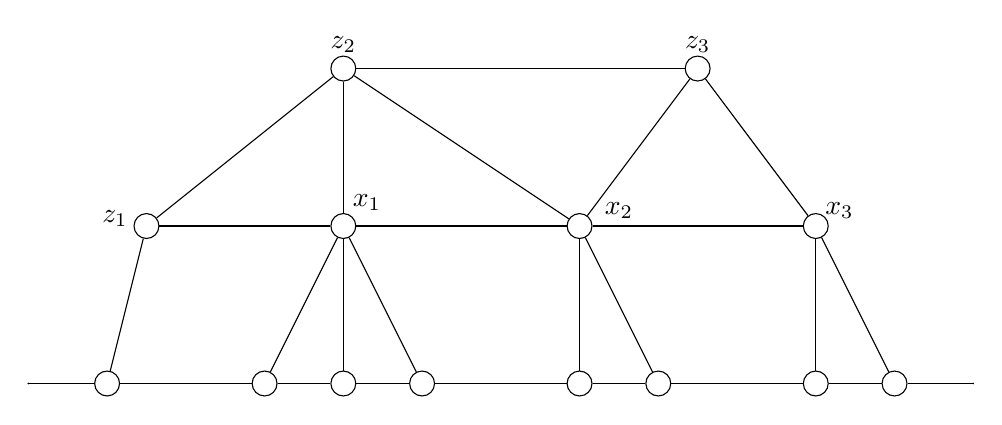
\begin{tikzpicture}
        \node[white] (1) at (1,0){};
        \node[white] (2) at (3,0){};
        \node[white] (3) at (4,0){};
        \node[white] (4) at (5,0){};
        \node[white] (5) at (7,0){};
        \node[white] (6) at (8,0){};
        \node[white] (7) at (10,0){};
        \node[white] (8) at (11,0){};
        \node[white] (9) at (1.5,2){};
        \node[] at (1.1,2.1){$z_1$};
        \node[white] (10) at (4,2){};
        \node[] at (4.3,2.3){$x_1$};
        \node[white] (11) at (7,2){};
        \node[] at (7.5,2.2){$x_2$};
        \node[white] (12) at (10,2){};
        \node[] at (10.3,2.2){$x_3$};
        \node[white] (13) at (4,4){};
        \node[] at (4,4.3){$z_2$};
        \node[white] (14) at (8.5,4){};
        \node[] at (8.5,4.3){$z_3$};
       \node[invisible] (15) at (0,0){};
        \node[invisible] (16) at (12,0){};

        \draw[black] (1)--(2);
        \draw[black] (2)--(3);
        \draw[black] (3)--(4);   
        \draw[black] (4)--(5); 
        \draw[black] (5)--(6); 
        \draw[black] (6)--(7); 
        \draw[black] (7)--(8); 
        \draw[black] (9)--(10);
        \draw[black] (10)--(11);
        \draw[black] (11)--(12);
        \draw[black] (13)--(14);

        \draw[black] (1)--(9);
        \draw[black] (2)--(10);
        \draw[black] (3)--(10);
        \draw[black] (4)--(10);
        \draw[black] (5)--(11);
        \draw[black] (6)--(11);
        \draw[black] (7)--(12);
        \draw[black] (8)--(12);

        \draw[black] (9)--(13);
        \draw[black] (10)--(13);
        \draw[black] (11)--(13);
        \draw[black] (11)--(14);
        \draw[black] (12)--(14);
        \draw[black] (15)--(1);  
        \draw[black] (16)--(8);  
        
\end{tikzpicture}
\caption{Vertices $z_1$, $z_2$, and $z_3$ as described in Claims \ref{x2nbrpath} and \ref{degx3}. For each $i \in \{1,2,3\}$, the vertex $x_i$ is in $X_i$. Moreover, $x_2$ is of type (1,0,0), and $x_3$ is of type (2,0,0).}
    \label{fig:z1z2z3}
\end{center}
\end{figure}








The following claim establishes that $\deg(x_2) = 6$. See Figure \ref{fig:z1z2z3} for an illustration of the vertices described in the claim. For the remainder of the proof, let $T_3 = T_2 \oplus x_3$, with $T_3 = (G_3, C_3, (L,M))$.

\begin{claim}\label{x2nbrpath}
The following both hold.
\begin{itemize}
    \item $\deg(x_2) = 6$, and
    \item there exist adjacent vertices $z_2, z_3 \not \in V(C)$ such that $z_2$ is adjacent to $x_2$ and $x_1$, and $z_3$ is adjacent to $x_2$ and $x_3$.
\end{itemize} 
\end{claim}
\begin{proof}
By Claim \ref{QuasiQuasiSame}, this holds unless $\deg(x_2) = 5$.  Let $z \in V(G_3) \setminus V(C_3)$ be a neighbour of $x_2$. We claim $G \setminus \{x_2z\}$ has a $C_3$-critical subgraph. To see this, we start by extending $\phi$ to a partial $(L,M)$-colouring of $C \cup C_3$ as follows: first, note that since $x_1 \in X_1$ is a tripod of $T$ by Claim \ref{X1claims} (1), Claim \ref{s} implies that $|S(x_1)| = 2$. Similarly, since $x_2$ is of type (1,0,0) by Claim \ref{x2type}, we have that Claim \ref{s} implies that $|S(x_2)| = 3$. Since $x_3$ is of type (2,0,0), again Claim \ref{s} implies that $|S(x_3)| = 3$. By Claim \ref{matchmin}, $|M_{x_1x_2}| = |M_{x_2x_3}| = 5$. Thus there exists a colour $c_1 \in S(x_1)$ and a colour $c_3 \in S(x_3)$ such that $x_2[x_1, c_1] = x_2[x_3, c_3]$. Set $\phi(x_i) = c_i$ for $i \in \{1,3\}$. If $\phi$ extends to an $(L,M)$-colouring $\phi'$ of $G_3\setminus x_2z$, then $\phi'$ extends to an $(L,M)$-colouring of $G$ by redefining $\phi'(x_2)$ to be a colour in $S(x_2) \setminus \{x_2[x_1, c_1], x_2[z, \phi'(z)]\}$. Since $|S(x_2)| = 3$, such a choice exists \textemdash a contradiction, since $\phi$ does not extend to $G$. Thus $\phi$ does not extend to an $(L,M)$-colouring of $G_3\setminus x_2z$, and thus by Proposition \ref{CriticalSubgraph}, we have that $G_3\setminus x_2z$ has a $C_3$-critical subgraph, $G_3'$. But then $G_3'$ is a proper $C_3$-critical subgraph of $G_3$ (since $x_2z \not \in E(G_3')$). Since $T_3$ is a $3$-relaxation of $T$, this contradicts Claim \ref{criticalrelaxations}.
\end{proof}

For the remainder of the proof, let $z_1,z_2,$ and $z_3$ be as in Claims \ref{degu} and \ref{x2nbrpath}.
\begin{claim}\label{z2z3vc}
Neither $z_2$ nor $z_3$ have a neighbour in $V(C)$.
\end{claim}
\begin{proof}
Note that $N(z_2) \cap V(C)= \emptyset$, as otherwise given the existence of $z_1$ and $z_3$, we have that $z_2$ is a strong dividing vertex of $T_1$, contradicting Claim \ref{dividingrelaxations}. Moreover, note that $\deg(x_3) \geq 5$ by Proposition \ref{Facts} (2); and so, given that $x_3$ is a tripod of $T_2$ by Claim \ref{X3claims}, there exists a vertex $q_1 \in N(x_3)$ such that $q_1,z_3,x_2$ is part of the cyclic ordering of the neighbours of $x_3$ and $q_1 \not \in V(C)$. Thus $N(z_3) \cap V(C) = \emptyset$ by Claim \ref{z2z3vc}, as otherwise given the existence of $z_2$ and $q_1$, we have that $z_3$ is a strong dividing vertex of $T_3$, contradicting Claim \ref{dividingrelaxations}.
\end{proof}
The following claim bounds $d(T)$ in terms of $d(T_3)$ and establishes that $\deg(x_3) = 6$.

\begin{claim}\label{degx3}
$\deg(x_3) = 6$ and $d(T) \geq d(T_3)-3\varepsilon$. 
\end{claim}
\begin{proof}
Suppose not. First suppose that $\deg(x_3) \geq 6$. Note that since $x_1$ is a tripod of $T$; since $x_2$ is a tripod of $T_1$; and since $x_3$ is a tripod of $T_2$, it follows that $\defc(T) = \defc(T_1) = \defc(T_2) = \defc(T_3)$. Moreover, by Claim \ref{v(T)}, $v(T_3) \geq 5$. Thus by the minimality of $T$, we have that $d(T_3) \geq 3-\gamma$. In addition, note that $v(T_3) = v(T_2)-1$, that $v(T_2) = v(T_1)-1$, and that $v(T_1) = v(T)-1$. Thus, letting $T_0 := T$, we have that
\begin{equation}\label{dtbound}
       d(T_{i-1}) = d(T_{i}) - \varepsilon + \alpha\left(b(T_{i})-b(T_{i-1})+q(T_i)-q(T_{i-1}) \right) 
\end{equation}
for each $i \in \{1,2,3\}$.

Let $z_3, x_2, u_1, u_2, q_1, q_2, \dots $ be the neighbours of $z_3$ listed in their cyclic order around $z_3$, where $\{u_1, u_2 \} \subseteq V(C)$. Let $R = N(x_3) \setminus \{z_3,x_2,u_1,u_2,q_1\}$. We claim no vertex  $r \in R$ is in the quasiboundary of $T_2$; otherwise, given the existence of $z_3$ and $q_1$, we have that $r$ is a strong dividing vertex of $T_3$, contradicting Claim \ref{dividingrelaxations}. 

Note that $R \subseteq B(T_3) \subseteq Q(T_3)$. Thus since $x_3 \in Q(T_2) \setminus Q(T_3)$ and $R \subseteq Q(T_3) \setminus Q(T_2)$, it follows from Equation \ref{dtbound} that $$d(T_2) \geq d(T_3)-\varepsilon + 2\alpha(|R|-1).$$ By Claims \ref{QuasiQuasiSame} and \ref{x2nbrpath}, $d(T) \geq d(T_2)-2\varepsilon$. 

Combining these results, we have that 
\begin{align*}
    d(T) &\geq d(T_2)-2\varepsilon \\
    &\geq (d(T_3)-\varepsilon + 2\alpha(|R|-1))-2\varepsilon.
\end{align*}
Suppose that $\deg(x_3) \geq 7$, and so that $|R| \geq 2$. Then  $d(T) \geq d(T_3)-3\varepsilon + 2\alpha$. Since $d(T_3) \geq 3-\gamma$, this implies $d(T) \geq 3-\gamma-3\varepsilon+2\alpha$. This is a contradiction, since $3\varepsilon \leq 2\alpha$ by (I1). Thus $|R| = 1$, and so $\deg(x_3)=6$ and $d(T) \geq d(T_3)-3\varepsilon$, as desired.

Suppose now that $\deg(x_3) < 6$, and so that $\deg(x_3) = 5$ by Proposition \ref{Facts} (2). Recall that by Claim \ref{X2claims} (1), $x_1$ is a tripod of $T$. It follows from Claim \ref{s} that $|S(x_1)| = 2$; and moreover since $x_2$ is a tripod of $T_1$ by Claim \ref{X2claims} (1), we have further that $|S(x_2)| =3$.  Thus there exists a colour $c_2 \in S(x_2)$ such that $x_1[x_2, c_2] \not \in S(x_1)$. Let $\phi(x_2) = c_2$. Note that $N(z_2) \cap V(C)= \emptyset$ by Claim \ref{z2z3vc}. Thus by Claim \ref{s}, $|S(x_2)| =5$, and so there exists two distinct colours $d_1$ and $d_2$  in $S(z_2)$ such that $x_1[z_2, d_i] \not \in S(x_1)$ and $x_2[z_2, d_i] \neq c_2$ for $i \in \{1,2\}$. 

Furthermore, $N(z_3) \cap V(C) = \emptyset$ by Claim \ref{z2z3vc}. Thus by Claim \ref{s}, $|S(z_3)| = 5$. It follows that there exists an $i \in \{1,2\}$ such that $S(z_3) \setminus (\{z_3[z_2, d_i], z_3[x_2, c_2]\} \cup \{z_3[x_3, c]: c \in S(x_3)\})$ is non-empty, since $|S(z_3)| = 5$ and $z_3[z_2, d_1] \neq z_3[z_2, d_2]$. Without loss of generality, suppose that $i = 1$.  Let $d_3 \in S(z_3) \setminus (\{z_3[z_2, d_i], z_3[x_2, c_2]\} \cup \{z_3(x_3, c): c \in S(x_3)\})$. Finally, let $\phi(z_2) = d_1$ and $\phi(z_3) = d_3$.

Let $C'$ be obtained from $C_3$ by deleting $x_2$ and adding the vertices $z_2,z_3$ as well as edges $x_1z_2, z_2z_3,$ and $z_3x_3$. Let $T' = T\langle C' \rangle =  (G', C', (L,M))$. We claim that $G'-\{x_3q_1, x_1z_1\}$ has a $C'$-critical subgraph. To see this, note that if $\phi$ extends to $G'-\{x_3q_1, x_1z_1\}$, then $\phi$ extends to an $(L,M)$-colouring of $G$ by redefining $\phi(x_1)$ as a colour in $S(x_1) \setminus x_1[z_1, \phi(z_1)]$ and $\phi(x_3)$ as a colour in $S(x_3) \setminus \{x_3[q_1, \phi(q_1)], x_3[x_2, c_2]\}$. Such choices exist, since $|S(x_1)| = 2$ and $|S(x_3)|= 3$ by Claim \ref{s} since $x_3$ has exactly two neighbours in $V(C)$ by Claims \ref{not201}-\ref{not212}. This contradicts the fact that $\phi$ does not extend to $G$.  Thus $\phi$ does not extend to an $(L,M)$-colouring of $G'-\{x_3q_1, x_1z_1\}$, and so by Proposition \ref{CriticalSubgraph} we have that $G'-\{x_3q_1, x_1z_1\}$ has a $C'$-critical subgraph $G''$. Note that $v(T') \geq 2$ by Claim \ref{v(T)}, and $|E(G') \setminus E(G'')| \geq 2$.  Moreover, we claim that $C'$ is chordless: this follows easily from the facts that $C$ is chordless by Claim \ref{Chord}; that neither $z_2$ nor $z_3$ have a neighbour in $V(C)$ by Claim \ref{z2z3vc}; that $x_1z_3 \not \in E(G)$ since $G$ is planar; and that $z_2x_3 \not \in E(G)$ since $z_3$ has degree at least five by Proposition \ref{Facts} (2). Thus $|E(G'') \setminus E(C')| \geq 2$.

By Claim \ref{ProperCrit} (3)  applied to $T'$ and $G''$, we find that $d(T') \geq 5-(2\alpha + \varepsilon) - \gamma$. Moreover, $v(T') = v(T_2)+3$, $b(T') \geq b(T_2)-3$, and similarly $q(T') \geq q(T_2)-3$. Thus $s(T') \geq s(T_2)-(3\varepsilon +6\alpha)$. Furthermore, $\defc(T') = \defc(T_2)+1$. Putting all of this together,
\begin{align*}
    5-(2\alpha + \varepsilon)-\gamma &\leq d(T') \\
    &\leq \defc(T')-s(T') \\
    &\leq (\defc(T_2)+1)-(s(T_2)-(3\varepsilon + 6\alpha)) \\
    &\leq d(T_2)+1+(3\varepsilon + 6\alpha),
\end{align*}
which implies that $d(T_2) \geq 4-\gamma -(8\alpha+4\varepsilon)$. By Claim \ref{QuasiQuasiSame}, $d(T) \geq d(T_2)-2\varepsilon$, and so $d(T) \geq 4-\gamma-(8\alpha +6\varepsilon)$. This is a contradiction, since $8\alpha+6\varepsilon \leq 1$ by (I2) and (I3).
\end{proof}

We will complete the proof of Theorem \ref{theorem:stronglinear} by showing that $x_3$ is not of type (2,0,0), thereby arriving at a contradiction. Before we do this, we need the following key claim which establishes some of the correspondence assignment in the graph near $x_3$.

\begin{claim}\label{keyclaim}
The following both hold. 
\begin{enumerate}
    \item [(i)] The vertex $z_1$ has exactly one neighbour in $V(C)$, and there do not exist colours $d_1 \in S(x_1)$ and $d_2 \in S(x_2)$ such that $z_2[x_1, d_1] = z_2[x_2, d_2]$.
    \item [(ii)] Let $T_1 = (G_1, C_1, (L,M))$.  Let $\phi(x_1) \in S(x_1)$, let $S'(v) = S(v)$ for all $v \in V(G') \setminus N(x_1)$, let $S'(v) = S(v) \setminus v[x_1, \phi(x_1)]$ for each $v \in N(x_1)$. The vertex $z_2$ has exactly one neighbour in $V(C')$. Moreover, there do not exist colours $d_2 \in S'(x_2)$ and $d_3 \in S'(x_3)$ such that $z_3[x_2, d_2] = z_3[x_3, d_3]$.
\end{enumerate}
\end{claim}

\begin{proof}
We begin by proving (i). First we will show that $z_1$ has exactly one neighbour in $V(C)$. To see this, suppose not. Since $z_1$ is in the boundary of $T$ by Claim \ref{degu}, it follows that $z_1$ has at least one neighbour in $V(C)$. Thus $z_1$ has at least two neighbours in $V(C)$. Since $x_1$ is adjacent to $z_1$ and there are no edges in $E(G)$ with both endpoints in $X_1$ by Claim \ref{X1claims} (3), it follows that that $z_1 \not \in X_1$ and so that $z_1$ has exactly two neighbours in $V(C)$. Thus by Claim \ref{s} we have that $|S(z_1)| = 3$. Similarly, since $x_2$ is a tripod of $T_1$ by Claim \ref{X2claims} (1), by Claim \ref{s}, $|S(x_2)| = 3$. Since $x_1$ is a tripod of $T$ by Claim \ref{X1claims} (1), we have further from Claim \ref{s} that $|S(x_1)| = 2$. Thus there exists a colour $c_1 \in S(z_1)$ and a colour $c_2 \in S(x_2)$ such that $x_1[z_1,c_1] \not \in S(x_1)$ and $x_1[x_2,c_2] \not \in S(x_1)$. Let $C' = C \oplus x_1 \oplus z_1 \oplus x_2$, and let $\phi(z_1) = c_1$ and $\phi(x_2) = c_2$. Let $T' = (G', C', (L,M)) = T\langle C' \rangle$. We claim $G' - x_1z_2$ has a $C'$-critical subgraph. To see this, note that if $\phi$ extends to an $(L,M)$-colouring of $G'-x_1z_2$, then by redefining $\phi(x_1)$ to be a colour in $S(x_1) \setminus x_1[z_2, \phi(z_2)]$ we obtain an extension of $\phi$ to an $(L,M)$-colouring of $G$, a contradiction. Thus $\phi$ does not extend to $G'-x_1z_2$, and so by Proposition \ref{CriticalSubgraph}, we have that $G'-x_1z_2$ contains a $C'$-critical subgraph $G''$. But $G''$ is a proper subgraph of $G'$, and $T'$ is a 3-relaxation of $T$. This contradicts Claim \ref{criticalrelaxations}.

Thus $z_1$ has exactly one neighbour in $V(C)$, and so by Claim \ref{s} we have that $|S(z_1)| = 4$. Since $|S(x_1)| =2$, there exist two distinct colours $c_1$ and $c_2$ in $S(z_1)$ with $x_1[z_1, c_1] \not \in S(x_1)$ and $x_1[z_1,c_2] \not \in S(x_1)$.

\begin{figure}[ht]
\tikzset{black/.style={shape=circle,draw=black,fill=black,inner sep=1pt, minimum size=9pt}}
\tikzset{white/.style={shape=circle,draw=black,fill=white,inner sep=1pt, minimum size=9pt}}

\tikzset{invisible/.style={shape=circle,draw=black,fill=black,inner sep=0pt, minimum size=0.1pt}}
\begin{center}
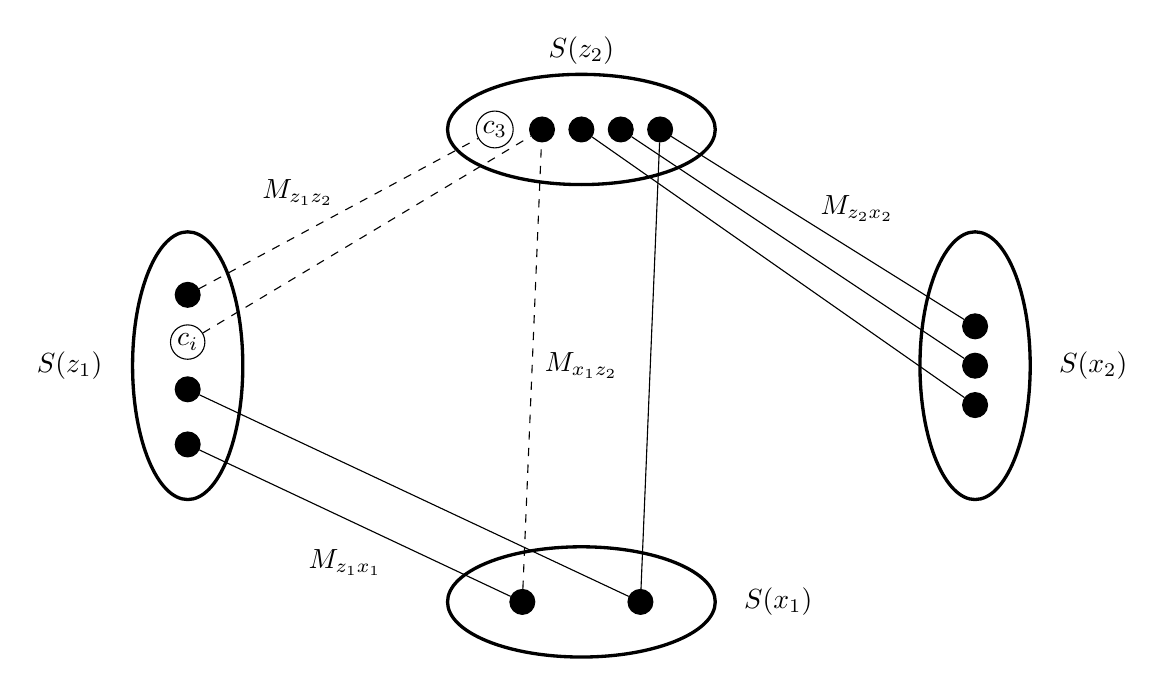
\begin{tikzpicture}
\filldraw[color=black!100, fill=black!0, very thick] (0,-3) ellipse (1.7 and 0.7);
\filldraw[color=black!100, fill=black!0, very thick] (5,0) ellipse (0.7 and 1.7);
\filldraw[color=black!100, fill=black!0, very thick] (-5,0) ellipse (0.7 and 1.7);
\filldraw[color=black!100, fill=black!0, very thick] (0,3) ellipse (1.7 and 0.7);
        \node[] at (-6.5,0) {$S(z_1)$};
        \node[] at (2.5,-3) {$S(x_1)$};
        \node[] at (6.5,0) {$S(x_2)$};
        \node[] at (0,4) {$S(z_2)$};
        
        \node[] at (0,0) {$M_{x_1z_2}$};
        \node[] at (-3.6,2.2) {$M_{z_1z_2}$};
        \node[] at (3.5,2) {$M_{z_2x_2}$};
        \node[] at (-3,-2.5) {$M_{z_1x_1}$};

        \node[black] (1) at (-5,0.9){};
        \node[white] (2) at (-5,0.3){$c_i$};
        \node[black] (3) at (-5,-0.3){};
        \node[black] (4) at (-5,-1){};
        \node[black] (5) at (-0.75,-3){};
        \node[black] (6) at (0.75,-3){};
        \node[black] (7) at (5,-0.5){};
        \node[black] (8) at (5,0){};
        \node[black] (9) at (5,0.5){};
        \node[black] (10) at (1,3){};
        \node[black] (11) at (0.5,3){};
        \node[black] (12) at (0,3){};
        \node[black] (13) at (-0.5,3){};
        \node[white] (14) at (-1.1,3){$c_3$};

        \draw[black] (3)--(6); 
        \draw[black] (4)--(5); 
        \draw[black] (6)--(10); 
        \draw[black] (9)--(10); 
        \draw[black] (8)--(11); 
        \draw[black] (7)--(12); 
        \draw[dashed] (5)--(13);
        \draw[dashed] (2)--(13);
        \draw[dashed] (1)--(14);

\end{tikzpicture}


\caption{The matchings between $S(x_1)$, $S(x_2)$, $S(z_1)$, and $S(z_2)$, as described in Claim \ref{keyclaim}. The matching $M_{x_2x_1}$ is omitted for clarity. We assume there exists a colour $d_1 \in S(x_1)$ and $d_2 \in S(x_2)$ such that $z_2[x_1,d_1] = z_2[x_2,d_2]$. Without loss of generality, we may assume that the solid edges in the matchings are as shown. No matter the remainder of the edges in $M_{z_1z_2}$ and $M_{x_1z_2}$, there exist colours $c_i \in S(z_1)$ and $c_3 \in S(z_2)$ such that $c_i$ is unmatched in $M_{x_1z_1}$, such that $c_3$ is unmatched in $M_{x_1z_2}$ and $M_{x_2z_2}$, and such that $c_3 \neq z_2[z_1, c_i]$.} 
    \label{fig:matchings1}
\end{center}
\end{figure}








We now proceed with the rest of the claim. Suppose for a contradiction that there exist $d_1 \in S(x_1)$ and $d_2 \in S(x_2)$ such that $z_2[x_1, d_1] = z_2[x_2, d_2]$. Since $z_2$ has no neighbours in $V(C)$ by Claim \ref{z2z3vc}, by Claim \ref{s} we have that $|S(z_2)| = 5$, and so there exists a colour $c_3 \in S(z_2)$ and an $i \in \{1,2\}$ such that $c_3 \neq z_2[z_1, c_i]$, such that $x_1[z_2, c_3] \not \in S(x_1)$, and such that $x_2[z_2, c_3] \not \in S(x_2)$: that is, there is a colour choice $c_i$ for $z_1$ that avoids $S(x_1)$, and a colour choice $c_3 \in S(z_2)$ that avoids $c_i \in S(z_1)$ as well as $S(x_1)$ and $S(x_2)$. See Figure \ref{fig:matchings1} for an illustration of the matchings described. Let $C''$ be obtained from $(C \oplus x_1 \oplus x_2) \setminus \{x_1\}$ by adding the vertices $z_1$ and $z_2$ as well as edges $yz_1,z_1z_2,z_2x_2$, where $y \in N(z_1) \cap V(C)$. Let $T'' = (G'', C'', (L,M)) = T \langle C'' \rangle$. Recall that $\deg(x_2) = 6$ by Claim \ref{X2claims} (2); and $N(x_2) \setminus (V(C'') \cup \{x_1\}) = \{z_3, x_3\}$.

We claim that $G'' \setminus \{x_2z_3, x_2x_3\}$ has a $C''$-critical subgraph. To see this, choose $\phi(z_1) = c_i$, and $\phi(z_2) = c_3$. If $\phi$ extends to an $(L,M)$-colouring of $G'' \setminus \{x_1, x_2\}$, then $\phi$ extends to an $(L,M)$-colouring of $G$ by first choosing $\phi(x_2) \in S(x_2) \setminus \{x_2[z_3, \phi(z_3)], x_2[x_3, \phi(x_3)]\}$, and then choosing $\phi(x_1) \in S(x_1) \setminus \{x_1[x_2, \phi(x_2)]\}$. Note this is possible, since $|S(x_1)| = 2$ and $|S(x_2)| = 3$. This is a contradiction, since $\phi$ does not extend to $G$ by assumption. Thus $\phi$ does not extend to an $(L,M)$-colouring of $G''-\{x_1, x_2\}$, and so by Proposition \ref{CriticalSubgraph} we have that $G'' \setminus \{x_2z_3, x_2x_3\}$ has a $C''$-critical subgraph. But then $G''$ contains a proper $C''$-critical subgraph $G^*$. Note that $|E(G'') \setminus E(G^*)| \geq 2$, and by Claim \ref{v(T)}, $v(T'') \geq 3$. Finally, we claim $|E(G^*) \setminus E(C'')| \geq 2$. To see this, note that since $C$ is chordless by Claim \ref{Chord}; since $z_1$ has exactly one neighbour $y$ in $V(C)$ as shown above; since neither $z_2$ nor $z_3$ have a neighbour in $V(C)$ by Claim \ref{z2z3vc}; and since $z_1x_2 \not \in E(G)$ since $G$ is planar, it follows that $C''$ is chordless. Thus $|E(G^*) \setminus E(C'')| \geq 2$. By Claim \ref{ProperCrit} (3) applied to $T''$ and $G^*$, we find that $d(T'') \geq 5-(2\alpha + \varepsilon) -\gamma$. In addition, $s(T_2) \leq s(T'')+2(2\alpha+\varepsilon)$, $\defc(T_2) \geq \defc(T'')-1$, and so $d(T_2) \geq d(T'')-1-2(2\alpha + \varepsilon)$. Thus $d(T_2) \geq 4-\gamma-3(2\alpha+\varepsilon)$. By Claim \ref{QuasiQuasiSame}, $d(T) \geq d(T_2)-2\varepsilon$ and so $d(T) \geq d(T_2)-2\varepsilon \geq 4-\gamma-(6\alpha+5\varepsilon)$. But then $d(T) \geq 3-\gamma$ since by (I2) and (I3) we have that $6\alpha+5\varepsilon \leq 1$. This contradicts the fact that $T$ is a counterexample.

The proof of (ii) is nearly identical. For each $uv \in E(G')$, let $M'_{uv}$ be the restriction of $M_{uv}$ to $S'(u)$ and $S'(v)$. Recall that by Claim \ref{matchmin}, we have that $|M_{z_2x_1}|=5$. Note that $z_2$ is not adjacent to a vertex in $V(C)$ by Claim \ref{z2z3vc}. Thus as $z_2$ is adjacent to $x_1$, we have that $z_2$ has exactly one neighbour in $V(C) \oplus x_1$, and so by Claim \ref{matchmin}, we have that $|S'(z_2)| = 4$. Similarly, $|S'(x_2) = 2|$. Thus there exist two colours $c_1, c_2 \in S'(z_2)$ such that for $i \in \{1,2\}$, we have that $x_2[x_2, c_i] \not \in S'(x_2)$.  Moreover, since $|S'(x_2)|=2$ and $|S'(z_3)|=5$, by Claim \ref{matchmin} we have that that $|M'_{x_2z_3}| = 2$. Recall that $|S(x_3)| = 2$ by Claim \ref{s} and that $|S(z_3)|=5$ by Claims \ref{z2z3vc} and \ref{s}. Since $G$ is planar, neither $x_3$ nor $z_3$ is adjacent to $x_1$. Thus $|M'_{x_3z_2}|= 3$. Suppose for a contradiction that there exist colours $d_2 \in S'(x_2)$ and $d_3 \in S'(x_3)$ such that $z_3[x_2, d_2] = z_3[x_3, d_3]$. Then there exists a colour $c_3 \in S'(z_3)$ and an $i \in \{1,2\}$ such that $c_3 \neq z_3[z_2, c_i]$, such that $x_2[z_3, c_3] \not \in S'(x_2)$, and such that $x_3[z_3, c_3] \not \in S'(x_3)$: that is, there is a colour choice $c_i$ for $z_2$ that avoids $S'(x_2)$, and a colour choice $c_3 \in S'(z_3)$ that avoids $c_i \in S'(z_2)$ as well as $S'(x_2)$ and $S'(x_3)$. See Figure \ref{fig:matchings2} for an illustration of the matchings involved. Let $C'$ be obtained from $(C_1 \oplus x_2 \oplus x_3) \setminus \{x_2\}$ by adding the vertices $z_2$ and $z_3$ as well as edges $x_1z_2,z_2z_3,z_3x_3$. Let $T' = T \langle C'' \rangle = (G', C', (L,M))$. Recall that $\deg(x_3) = 6$ by Claim \ref{degx3}. Let $N(x_3) \setminus (V(C) \cup \{x_2,z_3\}) = \{z_4, z_5\}$.

\begin{figure}[ht]
\tikzset{black/.style={shape=circle,draw=black,fill=black,inner sep=1pt, minimum size=9pt}}
\tikzset{white/.style={shape=circle,draw=black,fill=white,inner sep=1pt, minimum size=9pt}}

\tikzset{invisible/.style={shape=circle,draw=black,fill=black,inner sep=0pt, minimum size=0.1pt}}
\begin{center}
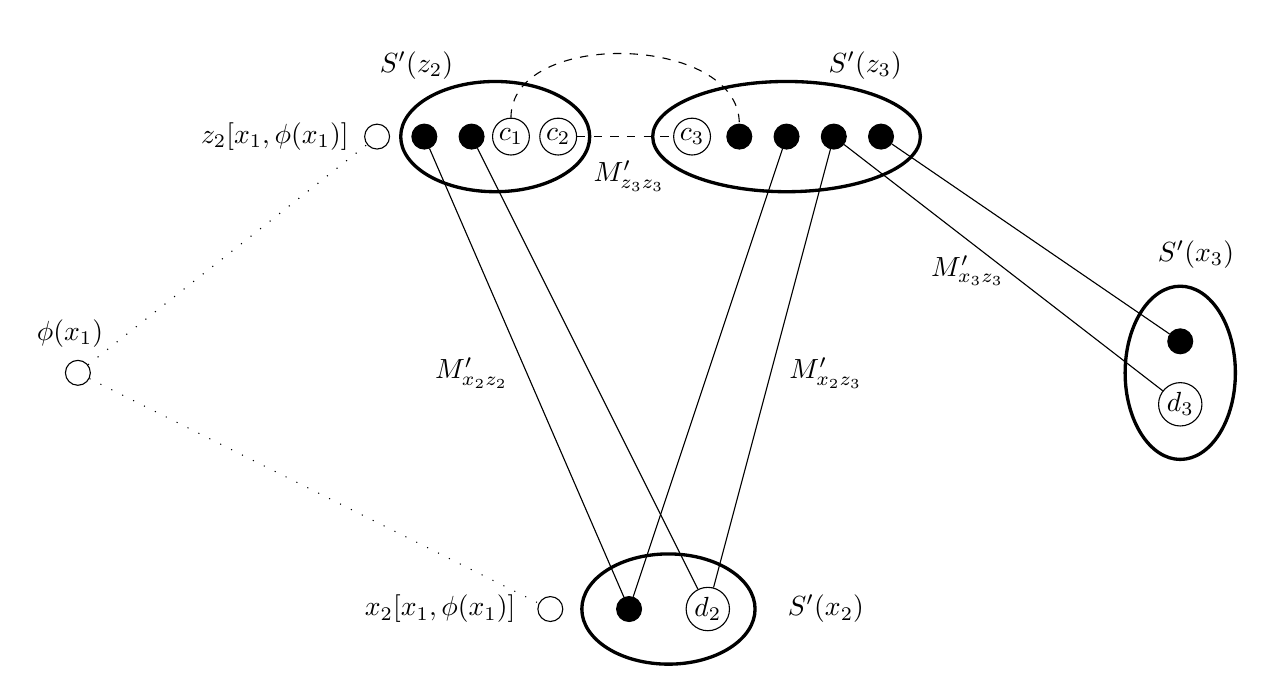
\begin{tikzpicture}
\filldraw[color=black!100, fill=black!0, very thick] (0.5,-3) ellipse (1.1 and 0.7);
\filldraw[color=black!100, fill=black!0, very thick] (7,0) ellipse (0.7 and 1.1);
%\filldraw[color=black!100, fill=black!0, very thick] (-7,0) ellipse (0.7 and 1.7);
\filldraw[color=black!100, fill=black!0, very thick] (-1.7,3) ellipse (1.2 and 0.7);
\filldraw[color=black!100, fill=black!0, very thick] (2,3) ellipse (1.7 and 0.7);

        %\node[] at (-8,0) {$x_1$};
        \node[] at (2.5,-3) {$S'(x_2)$};
        \node[] at (-2.7,3.9) {$S'(z_2)$};
        \node[] at (3,3.9) {$S'(z_3)$};
        \node[] at (7.2,1.5) {$S'(x_3)$};


        \node[white] (1) at (-7,0){};
        \node[white] (2) at (-3.2,3){};
        \node[black] (3) at (-2.6,3){};
        \node[black] (4) at (-2,3){};
        \node[white] (5) at (-1.5,3){$c_1$};
        \node[white] (6) at (-0.9,3){$c_2$};
        \node[white] (7) at (0.8,3){$c_3$};
        \node[black] (8) at (1.4,3){};
        \node[black] (9) at (2,3){};
        \node[black] (10) at (2.6,3){};
        \node[black] (11) at (3.2,3){};
        \node[black] (12) at (7,0.4){};
        \node[white] (13) at (7,-0.4){$d_3$};
        \node[white] (14) at (1,-3){$d_2$};
        \node[black] (15) at (0,-3){};
        \node[white] (16) at (-1,-3){};

        \node[] (17) at (-7.1,0.5){$\phi(x_1)$};
        \node[] at (-4.5,3) {$z_2[x_1, \phi(x_1)]$};
        \node[] at (-2.4,-3) {$x_2[x_1, \phi(x_1)]$};
        \node[] at (-2,0) {$M'_{x_2z_2}$};
        \node[] at (2.5,0) {$M'_{x_2z_3}$};
        \node[] at (4.3,1.3) {$M'_{x_3z_3}$};
        \node[] at (0,2.5) {$M'_{z_3z_3}$};



        \draw[loosely dotted] (1)--(2); 
        \draw[loosely dotted] (1)--(16); 
        \draw[black] (15)--(3); 
        \draw[black] (14)--(4); 
        \draw[black] (12)--(11); 
        \draw[black] (13)--(10); 
        \draw[black] (14)--(10); 
        \draw[black] (15)--(9); 
        \draw[out=90,in=90,dashed]  (5) to  (8);
        \draw[dashed] (6)--(7); 
        %\draw[black] (4)--(5); 
        %\draw[dashed] (2)--(13);
        %\draw[dashed] (1)--(14);

\end{tikzpicture}


\caption{The matchings between $S'(x_2)$, $S'(x_3)$, $S'(z_2)$, and $S'(z_3)$, as described in the proof of the second statement in Claim \ref{keyclaim}. The matching $M'_{x_2x_3}$ is omitted for clarity. We assume there exists a colour $d_2 \in S'(x_2)$ and $d_3 \in S'(x_3)$ such that $z_2[x_2,d_2] = z_2[x_3,d_3]$. Without loss of generality, we may assume that the solid edges in the matchings are as shown. No matter the matching $M'_{z_2z_3}$, there exist colours $c_i \in S'(z_2)$ and $c_3 \in S'(z_2)$ such that $c_i$ is unmatched in $M'_{x_2z_2}$, such that $c_3$ is unmatched in $M'_{x_2z_3}$ and $M'_{x_3z_3}$, and such that $c_3 \neq z_3[z_2, c_i]$.} 
    \label{fig:matchings2}
\end{center}
\end{figure}







We claim that $G' \setminus \{x_3z_4, x_3z_5\}$ has a $C'$-critical subgraph. To see this, choose $\phi(z_2) = c_i$, and $\phi(z_3) = c_3$. If $\phi$ extends to an $(L,M)$-colouring of $G' \setminus \{x_2, x_3\}$, then $\phi$ extends to an $(L,M)$-colouring of $G$ by first choosing $\phi(x_3) \in S'(x_3) \setminus \{x_3[z_4, \phi(z_4)], x_3[z_5, \phi(z_5)]\}$, and then choosing $\phi(x_2) \in S'(x_2) \setminus \{x_2[x_3, \phi(x_3)]\}$. Note this is possible, since $|S'(x_2)| = 2$ and $|S'(x_3)| = 3$. This is a contradiction, since $\phi$ does not extend to $G$ by assumption. Thus $\phi$ does not extend to an $(L,M)$-colouring of $G'-\{x_2, x_3\}$, and so by Proposition \ref{CriticalSubgraph} we have that $G' \setminus \{x_3z_4, x_3z_5\}$ has a $C'$-critical subgraph. But then $G'$ contains a proper $C'$-critical subgraph $G^*$. Note that $|E(G') \setminus E(G^*)| \geq 2$, and by Claim \ref{v(T)}, $v(T') \geq 3$. Finally, we claim that $C'$ is chordless: this follows from the facts that $C$ is chordless by Claim \ref{Chord}; that neither $z_2$ nor $z_3$ have neighbours in $V(C)$ by Claim \ref{z2z3vc}; and that $z_3z_1 \not \in V(C)$ since $G$ is planar. Thus $|E(G^*) \setminus E(C')| \geq 2$. By Claim \ref{ProperCrit} (3) applied to $T'$ and $G^*$, we find that $d(T') \geq 5-(2\alpha + \varepsilon) -\gamma$.

In addition, $s(T_3) \leq s(T')+2(2\alpha+\varepsilon)$, and $\defc(T_3) \geq \defc(T')-1$. Thus $d(T_3) \geq d(T')-1-2(2\alpha + \varepsilon)$, and so since  $d(T') \geq 5-(2\alpha + \varepsilon) -\gamma$, we have that  $d(T_3) \geq 4-\gamma-3(2\alpha+\varepsilon)$. By Claim \ref{degx3}, $d(T) \geq d(T_3)-3\varepsilon$. Thus $d(T) \geq 4-\gamma-6\alpha-6\varepsilon$. But this is a contradiction, since by (I2) and (I3) we have that $6\alpha+6\varepsilon \leq 1$.
\end{proof}

We now show $x_3$ is not of type (2,0,0), thus contradicting Claim \ref{x3type} and completing the proof of Theorem \ref{theorem:stronglinear}.

\begin{claim}\label{not200}
$x_3$ is not of type (2,0,0).
\end{claim}
\begin{proof}
Suppose not. By Claim \ref{X1claims} (1), we have that $x_1$ is a tripod of $T$. By Claim \ref{s}, it follows that $|S(x_1)| = 2$. Let $|S(x_1)| = \{c_1, c_2\}$, and for each $i \in \{1,2\}$, let $\phi_i$ be an extension of $\phi$ to $x_1$ with $\phi_i(x_1) = c_i$; let $S_i(x_2) = S(x_2) \setminus x_2[x_1, c_i]$; and similarly let $S_i(x_3) = S(x_3) \setminus x_3[x_1, c_i]$. Note that $S_1(x_2) \neq S_2(x_2)$ since $c_1$ and $c_2$ are distinct. Furthermore, note that $x_3$ is not adjacent to $x_1$ since $x_3$ is a tripod of $T_2$ of type (2,0,0): thus $S_i(x_3) = S(x_3)$ is a fixed set that does not depend on $i$. Let $M^i_{z_3x_2}$ be the restriction of $M_{z_3x_2} $ to $S_i(z_3)$ and $S_i(x_2)$.  Finally, let $S = S(z_3)\setminus \{z_3[x_3, d] : d \in S_i(x_3)\}$.  Since $S_i(x_3)$ is fixed, so too is $S$.

Note that by Claim \ref{matchmin}, we have that $|M^i_{z_3x_2}| = 2$ for each $i \in \{1,2\}$, and moreover by Claim \ref{keyclaim} (2) there does not exist a colour $d_3 \in S_i(x_3)$ and a colour $d_2 \in S_i(x_2)$ such that $z_3[x_2, d_2] = z_3[x_3, d_3]$.  Since $S$ is fixed, this implies that $M^1(z_3x_2) = M^2(z_3x_2)$. This is a contradiction, since $S_1(x_2)$ and $S_2(x_2)$ are distinct sets of size two.
\end{proof}

